


\documentclass[11pt]{article}

\usepackage[top=.85in, bottom=.65in, left=.56in, right=.45in, footskip=0pt,
paperheight=13.5in,paperwidth=9.25in]{geometry}

\usepackage{csquotes}

\newcommand{\Ldown}[1]{\hspace{-2pt}\raisebox{-1pt}{{%\fontfamily{lmhh}
\fontsize{14}{11}\selectfont{}{\textnormal{#1.}}}}\hspace{3pt}}


\newcommand{\semihr}[1]{{\textcolor{orange!60!black}{\hrule width #1}}}


\usepackage{xcolor}


\usepackage{xcolor}



%\input{commands}

\newcommand{\mdash}{---}
\newcommand{\q}[1]{``#1''}
\newcommand{\br}{

}

\newcommand{\raggedRightTitle}[1]{\br{}\begin{flushleft}\textbf{#1}\end{flushleft}}

%\newcommand{\visavis}{vis-\`a-vis}


%\input{ngml/ngml-setup-commands}
%\input{ngml/ngml-sdi-commands}
%\input{ngml/ngml-deco-commands}

%\AtEndDocument{\immediate\write18{cd /home/nlevisrael/gits/ntxh/wip-sebi/ar/code/cpp/qmake-console/projects/gtagml/ngml-sdi-console; ./run-with-args.sh /home/nlevisrael/gits/ntxh/wip-sebi/gtagml/ctg/gen/ctg/ctg.gt.tex /home/nlevisrael/gits/ntxh/wip-sebi/gtagml/ctg/gen/ctg/ctg.gt.sdi.ntxh /home/nlevisrael/gits/ntxh/wip-sebi/gtagml/ctg/gen/ctg/ctg.gt.sdi-prelatex.ntxh; cd -;}}



% pmml  arff  openannotation

\usepackage[T1]{fontenc}
\usepackage{tgtermes}

\usepackage[hang,flushmargin]{footmisc}

\usepackage{titlesec}

\titlespacing*{\section}
{0pt}{4ex plus 1ex minus .5ex}{.1ex plus .2ex}

%\usepackage{titlesec}

\titleformat{\section}
  {\normalfont\Large\bfseries}   % The style of the section title
  {}                             % a prefix
  {0pt}                          % How much space exists between the prefix and the title
  {} 


%\usepackage{mathptmx}

\usepackage{eso-pic}

\AddToShipoutPictureBG{%

\colorlet{redbl}{red!40!magenta}
\colorlet{yelbl}{yellow!60!magenta}

\colorlet{redblg}{redbl!30!black}

\ifnum\value{page}>66{
\AtTextLowerLeft{\raisebox{-21pt}{\hspace{-15pt}\fontfamily{qtm}\fontsize{10}{11}\fontseries{b}\selectfont{}{\colorbox{yelbl!7}{\textcolor{redblg!70}{PLEASE SEE OUR SOFTWARE DEMO VIDEOS: \href{http://www.lingtechsys.com/videos/qmt-composite.mkv}{GIS},
\href{http://www.lingtechsys.com/videos/dhax-composite.mkv}{360\textdegree{} photography}, and \href{http://www.lingtechsys.com/videos/xcsd-composite.mkv}{image processing}.}}}}}
}\fi
}


%\setlength\parindent{0pt}

\AddToShipoutPictureBG{%

\ifnum\value{page}>1{
\AtTextUpperLeft{
\makebox[23.1cm][r]{
\raisebox{-.6cm}{%
{\transparent{0.3}{
\includegraphics[width=0.19\textwidth]{e-logo.png}}	}} } }
}\fi
}

\AddToShipoutPicture{%
{
 {\color{blGreen!70!red}\transparent{0.9}{\put(0,0){\rule{3pt}{\paperheight}}}}%
 {\color{darkRed!70!purple}\transparent{1}\put(3,0){{\rule{4pt}{\paperheight}}}}
% {\color{logoPeach!80!cyan}\transparent{0.5}{\put(0,700){\rule{1cm}{.6cm}}}}%
% {\color{darkRed!60!cyan}\transparent{0.7}\put(0,706){{\rule{1cm}{.6cm}}}}
% \put(18,726){\thepage}
% \transparent{0.8}
}
}

%\AddToShipoutPicture{%
%\ifnum\value{page}=1
%\put(247.5,988){%
%	\transparent{0.7}{
%		\includegraphics[width=0.4\textwidth]{logo.png}}}
%\fi
%}	


\AddToShipoutPictureBG{%
\ifnum\value{page}=14

\put(7,678){
	\transparent{1}{
		\includegraphics[angle=0.5,origin=c,width=0.4\textwidth]{pm/1a.jpg}}}


\put(241,698){
	\transparent{1}{
		\includegraphics[angle=0,origin=c,width=0.31\textwidth,
trim=0 14mm 0 10mm, clip]{pm/7a.png}}}


\put(6,492){
	\transparent{1}{
		\includegraphics[angle=-0.5,origin=c,width=0.4\textwidth]{pm/5a.png}}}


\put(452,712){
	\transparent{1}{
		\includegraphics[angle=-1,origin=c,width=0.3\textwidth]{pm/2a.png}}}



\put(442,681){
	\transparent{1}{
		\includegraphics[angle=0,origin=c,width=0.18\textwidth]{pm/8a.png}}}


%\put(412,680){
%	\transparent{1}{
%		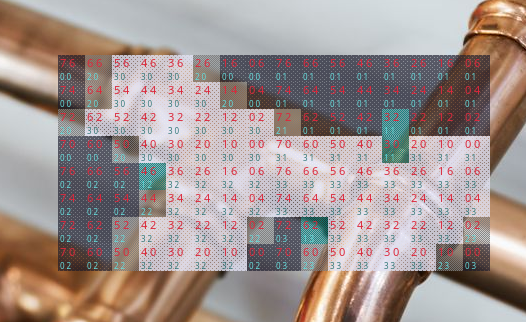
\includegraphics[angle=2.5,origin=c,width=0.2\textwidth]{pm/8.png}}}


\put(402,487){
	\transparent{1}{
		\includegraphics[angle=-1,origin=c,width=0.45\textwidth]{pm/3a.jpg}}}

\fi
}	




%\pagestyle{empty} % no page number
%\parskip 7.2pt    % space between paragraphs
%\parindent 12pt   % indent for new paragraph
%\textwidth 4.5in  % width of text
%\columnsep 0.8in  % separation between columns

%\setlength{\footskip}{-3pt}

%\usepackage[paperheight=15in,paperwidth=8.5in]{geometry}
%\geometry{left=.65in,top=.65in,right=.45in,bottom=1.25in} %margins

%\renewcommand{\thepage}{\raisebox{2pt}{\arabic{page}}}

\renewcommand{\footnoterule}{%
	\kern -3pt
	\hrule width .92\textwidth height .5pt
	\kern 10pt
}


\usepackage[hyphens]{url}
\newcommand{\biburl}[1]{ {\fontfamily{gar}\selectfont{\textcolor[rgb]{.2,.6,0}%
{\scriptsize {\url{#1}}}}}}

\newcommand{\bhref}[1]{\href{#1}{#1}}



%\linespread{1.3}

\newcommand{\sectsp}{\vspace{12pt}}

\usepackage{graphicx}
\usepackage{color,framed}

\usepackage{textcomp}

\usepackage{float}

\usepackage{mdframed}


\usepackage{setspace}

\usepackage{xcolor}

\usepackage[hyphenbreaks]{breakurl}
\usepackage[hyphens]{url}

%\usepackage{hyperref}

\colorlet{blCyan}{cyan!50!blue}

\definecolor{darkRed}{rgb}{.2,.0,.1}


\definecolor{blGreen}{rgb}{.2,.7,.3}

\definecolor{darkBlGreen}{rgb}{.1,.3,.2}

\definecolor{oldBlColor}{rgb}{.2,.7,.3}

\definecolor{blColor}{rgb}{.1,.3,.2}

\definecolor{elColor}{rgb}{.2,.1,0}
\definecolor{flColor}{rgb}{0.7,0.3,0.3}

\definecolor{logoOrange}{RGB}{108, 18, 30}
\definecolor{logoGreen}{RGB}{85, 153, 89}
\definecolor{logoPurple}{RGB}{200, 208, 30}

\definecolor{logoBlue}{RGB}{4, 2, 25}
\definecolor{logoPeach}{RGB}{255, 159, 102}
\definecolor{logoCyan}{RGB}{66, 206, 244}
\definecolor{logoRed}{rgb}{.3,0,0}

\newcommand{\colorq}[1]{{\color{logoOrange!70!black}{\q{\small\textbf{#1}}}}}

\let\qq\q

\definecolor{inOne}{rgb}{0.122, 0.435, 0.698}% Rule colour
\definecolor{inTwo}{rgb}{0.122, 0.698, 0.435}% Rule colour

\definecolor{outOne}{rgb}{0.435, 0.698, 0.122}% Rule colour
\definecolor{outTwo}{rgb}{0.698, 0.435, 0.122}% Rule colour

\colorlet{linkcolor}{flColor!60!red}




\usepackage[many]{tcolorbox}% http://ctan.org/pkg/tcolorbox

\usepackage{transparent}

\newlength{\bsep}
\setlength{\bsep}{-1pt}
\let\xbibitem\bibitem
\renewcommand{\bibitem}[2]{\vspace{\bsep}\xbibitem{#1}{#2}}

\newenvironment{cframed}{\begin{mdframed}[linecolor=logoPeach,linewidth=0.4mm]}{\end{mdframed}}

\newenvironment{ccframed}{\begin{mdframed}[backgroundcolor=logoGreen!5,linecolor=logoCyan!50!black,linewidth=0.4mm]}{\end{mdframed}}

\usepackage{aurical}
\usepackage[T1]{fontenc}

\usepackage{relsize}

\newcommand{\bref}[1]{\hspace*{1pt}\textbf{\ref{#1}}}

\newcommand{\dashsep}{--\hspace*{5pt}}

\newcommand{\pseudoIndent}{

\vspace{2pt}\hspace*{6pt}}

\usepackage{titlesec}

\titlespacing*{\subsection}
{0pt}{5ex plus 1ex minus .2ex}{0.5ex plus .2ex}


%\titlespacing*{\section}
%{0pt}{3.5ex plus 1ex minus .2ex}{1ex plus .2ex}

%
\newcommand{\deconum}[1]{{\protect\raisebox{-1pt}{{\LARGE #1}}}}

\newcommand{\visavis}{vis-\`a-vis}

\newcommand{\VersatileUX}{{\color{red!85!black}{\Fontauri Versatile}}%
{{\fontfamily{qhv}\selectfont\smaller UX}}}

\newcommand{\NDPCloud}{{\color{red!15!black}%
{\fontfamily{qhv}\selectfont {\smaller NDP C{\smaller LOUD}}}}}

\newcommand{\MThreeK}{{\color{blGreen!45!black}%
{\fontfamily{qhv}\fontsize{10}{8}\selectfont {M3K}}}}


\newcommand{\lfNDPCloud}{{\color{red!15!black}%
{\fontfamily{qhv}\selectfont N{\smaller DP C{\smaller LOUD}}}}}

\newcommand{\textds}[1]{{\fontfamily{lmdh}\selectfont{%
\raisebox{-1pt}{#1}}}}

\newcommand{\dsC}{{\textds{ds}{\fontfamily{qhv}\selectfont \raisebox{-1pt}
{\color{red!15!black}{C}}}}}

\definecolor{tcolor}{RGB}{24,52,61}

\newcommand{\CCpp}{\resizebox{!}{7pt}{\AcronymText{C}}/\Cpp{}}
\newcommand{\NoSQL}{\resizebox{!}{6.5pt}{\AcronymText{NoSQL}}}
\newcommand{\SQL}{\resizebox{!}{7pt}{\AcronymText{SQL}}}

\newcommand{\NCBI}{\resizebox{!}{7pt}{\AcronymText{NCBI}}}
\newcommand{\BioNetGen}{\resizebox{!}{7pt}{\AcronymText{BioNetGen}}}
\newcommand{\BNGL}{\resizebox{!}{7pt}{\AcronymText{BNGL}}}

\newcommand{\GML}{\resizebox{!}{7pt}{\AcronymText{GML}}}

\newcommand{\GIS}{\resizebox{!}{6.5pt}{\AcronymText{GIS}}}
\newcommand{\ACRIS}{\resizebox{!}{6.5pt}{\AcronymText{ACRIS}}}
\newcommand{\HPD}{\resizebox{!}{6.5pt}{\AcronymText{HPD}}}


\newcommand{\HTXN}{\resizebox{!}{7pt}{\AcronymText{HTXN}}}

\newcommand{\TDM}{\resizebox{!}{7pt}{\AcronymText{TDM}}}

\newcommand{\lHTXN}{\resizebox{!}{7.5pt}{\AcronymText{H}}%
\resizebox{!}{6.5pt}{\AcronymText{TXN}}}

\newcommand{\lsHTXN}{\resizebox{!}{9.5pt}{\AcronymText{\textcolor{tcolor}{HTXN}}}}

\newcommand{\LAF}{\resizebox{!}{7pt}{\AcronymText{LAF}}}

\newcommand{\UDpipe}{\resizebox{!}{7pt}{\AcronymText{UDpipe}}}

\newcommand{\C}{\resizebox{!}{7pt}{\AcronymText{C}}}

\newcommand{\TME}{\resizebox{!}{7pt}{\AcronymText{TME}}}

\newcommand{\TwoD}{\resizebox{!}{6.5pt}{\AcronymText{2D}}}




\usepackage{mdframed}

\newcommand{\cframedboxpanda}[1]{\begin{mdframed}[linecolor=yellow!70!blue,linewidth=0.4mm]#1\end{mdframed}}





\newcommand{\libSBML}{\resizebox{!}{7pt}{\AcronymText{libSBML}}}


\newcommand{\PVD}{\resizebox{!}{7pt}{\AcronymText{PVD}}}


\newcommand{\SDK}{\resizebox{!}{7pt}{\AcronymText{SDK}}}
\newcommand{\NLP}{\resizebox{!}{7pt}{\AcronymText{NLP}}}


\newcommand{\PDF}{\resizebox{!}{6.5pt}{\AcronymText{PDF}}}
\newcommand{\TEI}{\resizebox{!}{7.5pt}{\AcronymText{TE{\hspace*{.5pt}I}}}}
\newcommand{\SSML}{\resizebox{!}{7.5pt}{\AcronymText{SSML}}}
\newcommand{\ToBI}{\resizebox{!}{7.5pt}{\AcronymText{ToBI}}}

\newcommand{\MMBioS}{\resizebox{!}{6.5pt}{\AcronymText{MMBioS}}}

\newcommand{\VTK}{\resizebox{!}{6.5pt}{\AcronymText{VTK}}}


\newcommand{\AXF}{\resizebox{!}{7pt}{\AcronymText{AXF}}}

\newcommand{\HyperGraphDB}{\resizebox{!}{7pt}{\AcronymText{HyperGraphDB}}}


\newcommand{\lAXF}{\resizebox{!}{7.5pt}{\AcronymText{A}}%
\resizebox{!}{6.5pt}{\AcronymText{XF}}}


\newcommand{\lsAXF}{\resizebox{!}{8.5pt}{\AcronymText{AXF}}}

\newcommand{\AXFD}{\resizebox{!}{7pt}{\AcronymText{AXFD}}}

\newcommand{\lAXFD}{\resizebox{!}{7.5pt}{\AcronymText{A}}%
\resizebox{!}{6.5pt}{\AcronymText{XFD}}}


\newcommand{\IJST}{\resizebox{!}{7pt}{\AcronymText{IJST}}}

\newcommand{\BioC}{\resizebox{!}{7pt}{\AcronymText{BioC}}}

\newcommand{\CoNLL}{\resizebox{!}{7pt}{\AcronymText{CoNLL}}}
\newcommand{\CoNLLU}{\resizebox{!}{7pt}{\AcronymText{CoNLL-U}}}


\newcommand{\ePub}{\resizebox{!}{7pt}{\AcronymText{ePub}}}

%\lsLPF

\definecolor{atcColor}{RGB}{96, 17, 12}
%\textcolor{tcolor}{

\newcommand{\ATextCClr}[1]{\textcolor{atcColor}{\textbf{#1}}}

\newcommand{\ATexttclr}[1]{\textcolor{tcolor}{\textbf{#1}}}
\newcommand{\THQL}{\resizebox{!}{6.5pt}{\ATexttclr{THQL}}}


\newcommand{\ATextbk}[1]{\textcolor{black!50!cyan}{\textbf{#1}}}


%\newcommand{\lDHOS}{\resizebox{!}{7pt}{\ATexttclr{D}}%
%resizebox{!}{6.5pt}{\ATexttclr{HOS}}}

\newcommand{\PGVM}{\resizebox{!}{6.5pt}{\ATexttclr{PGVM}}}
\newcommand{\lPGVM}{\resizebox{!}{7pt}{\ATexttclr{PGVM}}}

\newcommand{\DHOS}{\resizebox{!}{6.5pt}{\ATexttclr{DHOS}}}
\newcommand{\lDHOS}{\resizebox{!}{7.5pt}{\ATexttclr{D}}\resizebox{!}{6.5pt}{\ATexttclr{HOS}}}
\newcommand{\sDHOS}{\resizebox{!}{6.5pt}{\ATexttclr{DHOS}}}

\newcommand{\sQt}{\resizebox{!}{6.5pt}{\ATexttclr{Qt}}}

\newcommand{\sPhVM}{\resizebox{!}{6.5pt}{\ATexttclr{P\hspace{.5pt}\textit{h}\hspace*{-.5pt}VM}}}


\newcommand{\PhVM}{\resizebox{!}{6.5pt}{\ATexttclr{P\hspace{.5pt}\textit{h}\hspace*{-.5pt}VM}}}
\newcommand{\lPhVM}{\resizebox{!}{7.5pt}{\ATexttclr{P}}\resizebox{!}{6.5pt}{\ATexttclr{\hspace{1pt}\textit{h}\hspace*{-.5pt}VM}}}


\newcommand{\MOC}{\resizebox{!}{7pt}{\AcronymText{MOC}}}
\newcommand{\SPARQL}{\resizebox{!}{7pt}{\AcronymText{SPARQL}}}
\newcommand{\GraphQL}{\resizebox{!}{7pt}{\AcronymText{GraphQL}}}

%{}, \QML{}, \GraphQL

\newcommand{\CCi}{\resizebox{!}{6.5pt}{\ATexttclr{CCi}}}
\newcommand{\XCSD}{\resizebox{!}{6.5pt}{\ATexttclr{XCSD}}}

\newcommand{\lXCSD}{\resizebox{!}{7pt}{\ATexttclr{XCSD}}}
\newcommand{\lCCi}{\resizebox{!}{7pt}{\ATexttclr{CCi}}}

%\newcommand{\ConceptsDB}{\resizebox{!}{6.5pt}{\ATexttclr{ConceptsDB}}}
%\newcommand{\lConceptsDB}{\resizebox{!}{7pt}{\ATexttclr{C}}\resizebox{!}{6.5pt}%{\ATexttclr{onceptsDB}}}


\newcommand{\GIT}{\resizebox{!}{7pt}{\AcronymText{GIT}}}

\newcommand{\LPF}{\resizebox{!}{7pt}{\AcronymText{LPF}}}
\newcommand{\lLPF}{\resizebox{!}{8.5pt}{\AcronymText{LPF}}}
\newcommand{\lsLPF}{\resizebox{!}{9.5pt}{\AcronymText{LPF}}}

\makeatletter

\newcommand*\getX[1]{\expandafter\getX@i#1\@nil}

\newcommand*\getY[1]{\expandafter\getY@i#1\@nil}
\def\getX@i#1,#2\@nil{#1}
\def\getY@i#1,#2\@nil{#2}
\makeatother
	
\newcommand{\rectann}[9]{%
\path [draw=#1,draw opacity=#2,line width=#3, fill=#4, fill opacity = #5, even odd rule] %
(#6) rectangle(\getX{#6}+#7,\getY{#6}+#8)
({\getX{#6}+((#7-(#7*#9))/2)},{\getY{#6}+((#8-(#8*#9))/2)}) rectangle %
({\getX{#6}+((#7-(#7*#9))/2)+#7*#9},{\getY{#6}+((#8-(#8*#9))/2)+#8*#9});}


\definecolor{pfcolor}{RGB}{94, 54, 73}

\newcommand{\EPF}{\resizebox{!}{7pt}{\AcronymText{ETS{\color{pfcolor}pf}}}}
\newcommand{\lEPF}{\resizebox{!}{8.5pt}{\AcronymText{ETS{\color{pfcolor}pf}}}}
\newcommand{\lsEPF}{\resizebox{!}{9.5pt}{\AcronymText{ETS{\color{pfcolor}pf}}}}

\newcommand{\RGB}{\resizebox{!}{6.5pt}{\AcronymText{RGB}}}


\newcommand{\GRE}{\resizebox{!}{7pt}{\AcronymText{GRE}}}
\newcommand{\CAS}{\resizebox{!}{7pt}{\AcronymText{CAS}}}

\newcommand{\lMOSAIC}{%
\resizebox{!}{8pt}{\AcronymText{M}}%
\resizebox{!}{6.5pt}{\AcronymText{OSAIC}}}

\newcommand{\XML}{\resizebox{!}{7pt}{\AcronymText{XML}}}
\newcommand{\RDF}{\resizebox{!}{7pt}{\AcronymText{RDF}}}
\newcommand{\DOM}{\resizebox{!}{7pt}{\AcronymText{DOM}}}


\newcommand{\CWL}{\resizebox{!}{7pt}{\AcronymText{CWL}}}




\newcommand{\Covid}{\resizebox{!}{7pt}{\AcronymText{Covid-19}}}

\newcommand{\CLang}{\resizebox{!}{7pt}{\AcronymText{C}}}

\newcommand{\HNaN}{\resizebox{!}{7pt}{\AcronymText{HN%
\textsc{a}N}}}

\newcommand{\JSON}{\resizebox{!}{7pt}{\AcronymText{JSON}}}

\newcommand{\MeshLab}{\resizebox{!}{7pt}{\AcronymText{MeshLab}}}
%\newcommand{\IQmol}{\resizebox{!}{7pt}{\AcronymText{IQmol}}}

\newcommand{\SGML}{\resizebox{!}{7pt}{\AcronymText{SGML}}}

\newcommand{\ASCII}{\resizebox{!}{7pt}{\AcronymText{ASCII}}}



\newcommand{\JATS}{\resizebox{!}{7pt}{\AcronymText{JATS}}}


\newcommand{\SDI}{\resizebox{!}{7pt}{\AcronymText{SDI}}}
\newcommand{\SDIV}{\resizebox{!}{7pt}{\AcronymText{SDIV}}}

\newcommand{\VXL}{\resizebox{!}{7pt}{\AcronymText{VXL}}}
\newcommand{\IQmol}{\resizebox{!}{7pt}{\AcronymText{IQmol}}}




\newcommand{\VM}{\resizebox{!}{7pt}{\AcronymText{VM}}}
\newcommand{\sVM}{\resizebox{!}{6.5pt}{\AcronymText{VM}}}


\newcommand{\IDE}{\resizebox{!}{7pt}{\AcronymText{IDE}}}


\newcommand{\OS}{\resizebox{!}{7pt}{\AcronymText{OS}}}

\newcommand{\FAIR}{\resizebox{!}{7pt}{\AcronymText{FAIR}}}
\newcommand{\FAIRsharing}{\resizebox{!}{7pt}{\AcronymText{FAIR}}\hspace*{1pt}\resizebox{!}{8pt}{sharing}}

\newcommand{\Python}{\resizebox{!}{7pt}{\AcronymText{Python}}}
\newcommand{\RPC}{\resizebox{!}{7pt}{\AcronymText{RPC}}}

\newcommand{\Java}{\resizebox{!}{7pt}{\AcronymText{Java}}}

\newcommand{\sBioNetGen}{\resizebox{!}{6.5pt}{\AcronymText{BioNetGen}}}
\newcommand{\sUI}{\resizebox{!}{6.5pt}{\AcronymText{UI}}}
\newcommand{\sAPOLLO}{\resizebox{!}{6.5pt}{\AcronymText{APOLLO}}}
\newcommand{\sSDK}{\resizebox{!}{6.5pt}{\AcronymText{SDK}}}
\newcommand{\sGUI}{\resizebox{!}{6.5pt}{\AcronymText{GUI}}}
\newcommand{\sAPI}{\resizebox{!}{6.5pt}{\AcronymText{API}}}




\newcommand{\QNetworkManager}{\resizebox{!}{7pt}{\AcronymText{QNetworkManager}}}
\newcommand{\QTextDocument}{\resizebox{!}{7pt}{\AcronymText{QTextDocument}}}

\newcommand{\QWebEngineView}{\resizebox{!}{6.5pt}{\AcronymText{QWebEngineView}}}

\newcommand{\HTTP}{\resizebox{!}{6.5pt}{\AcronymText{HTTP}}}


\newcommand{\lAcronymTextNC}[2]{{\fontfamily{fvs}\selectfont {\Large{#1}}{\large{#2}}}}

\newcommand{\AcronymTextNC}[1]{{\fontfamily{fvs}\selectfont {\large #1}}}



\colorlet{orr}{orange!60!red}

\colorlet{orb}{green!60!blue}
\colorlet{orbb}{green!30!blue}



\newcommand{\usstitle}[1]{\vspace{.4em}\raisebox{-1.2em}{{\fontfamily{gar}\fontsize{12}{14}%
\fontseries{sb}\selectfont{{\textcolor{orbb!65!black}{#1}}}}}}}


\newcommand{\sstitle}[1]{\vspace{1.4em}\raisebox{-1.2em}{{\fontfamily{gar}\fontsize{12}{14}%
\fontseries{sb}\selectfont{{\textcolor{orbb!65!black}{#1}}}}}}}

\newcommand{\DaSemio}{{\fontfamily{fvs}\fontsize{9}{14}%
\selectfont{\textbf{\textcolor{orb!75!black}{Da\resizebox{6pt}{!}{S}emio}}}}}}


\newcommand{\lDaSemio}{{\fontfamily{fvs}\fontsize{9}{14}%
\selectfont{\textbf{\textcolor{orb!75!black}{\resizebox{9pt}{!}{D}aSemio}}}}}}


%\newcommand{\DaSemio}{DaSemio}



\newcommand{\textscci}[1]{{\color{orr!35!black}{{%
						\fontfamily{Cabin-TLF}\fontseries{b}\selectfont{\textit{\scriptsize{#1}}}}}}}


\newcommand{\textscc}[1]{{\color{orr!35!black}{{%
						\fontfamily{Cabin-TLF}\fontseries{b}\selectfont{\textsc{\scriptsize{#1}}}}}}}


\newcommand{\textsccserif}[1]{{\color{orr!35!black}{{%
				\scriptsize{\textbf{#1}}}}}}


\newcommand{\iEPF}{\resizebox{!}{7pt}{\textsccserif{%
\textit{ETSpf}}}}

\newcommand{\iSDI}{\resizebox{!}{7pt}{\textsccserif{%
\textit{SDI}}}}

\newcommand{\iHTXN}{\resizebox{!}{7pt}{\textsccserif{%
\textit{HTXN}}}}




\newcommand{\AcronymText}[1]{{\textscc{#1}}}
\newcommand{\iAcronymText}[1]{{\textscci{#1}}}

\newcommand{\AcronymTextser}[1]{{\textsccserif{#1}}}


\newcommand{\mAcronymText}[1]{{\textscc{\normalsize{#1}}}}

\newcommand{\FASTA}{{\resizebox{!}{7pt}{\AcronymText{FASTA}}}}
\newcommand{\SRA}{{\resizebox{!}{7pt}{\AcronymText{SRA}}}}
\newcommand{\DNA}{{\resizebox{!}{7pt}{\AcronymText{DNA}}}}
\newcommand{\MAP}{{\resizebox{!}{7pt}{\AcronymText{MAP}}}}
\newcommand{\EPS}{{\resizebox{!}{7pt}{\AcronymText{EPS}}}}

\newcommand{\CSV}{{\resizebox{!}{6.5pt}{\AcronymText{CSV}}}}

%\newcommand{\PDB}{{\resizebox{!}{7pt}{\AcronymText{PDB}}}}


\newcommand{\APOLLO}{{\resizebox{!}{7pt}{\AcronymText{APOLLO}}}}
\newcommand{\GDC}{{\resizebox{!}{7pt}{\AcronymText{GDC}}}}
\newcommand{\TCIA}{{\resizebox{!}{7pt}{\AcronymText{TCIA}}}}
\newcommand{\CPTAC}{{\resizebox{!}{7pt}{\AcronymText{CPTAC}}}}





\newcommand{\XOCS}{{\resizebox{!}{7pt}{\AcronymText{XOCS}}}}


\newcommand{\cytoLib}{{\resizebox{!}{7pt}{\AcronymText{cytoLib}}}}
\newcommand{\CaPTk}{{\resizebox{!}{7pt}{\AcronymText{CaPTk}}}}
\newcommand{\DCMTK}{{\resizebox{!}{7pt}{\AcronymText{DCMTK}}}}
%\newcommand{\VM}{{\resizebox{!}{7pt}{\AcronymText{VM}}}}
\newcommand{\DSL}{{\resizebox{!}{7pt}{\AcronymText{DSL}}}}
\newcommand{\Paraview}{{\resizebox{!}{7pt}{\AcronymText{ParaView}}}}
\newcommand{\BFP}{{\resizebox{!}{7pt}{\AcronymText{BFP}}}}





\newcommand{\ChemXML}{{\resizebox{!}{7pt}{\AcronymText{ChemXML}}}}

\newcommand{\TeXMECS}{\resizebox{!}{7pt}{\AcronymText{TeXMECS}}}

% pmml  arff  openannotation

\newcommand{\PMML}{\resizebox{!}{7pt}{\AcronymText{PMML}}}
\newcommand{\ARFF}{\resizebox{!}{7pt}{\AcronymText{ARFF}}}
\newcommand{\IeXML}{\resizebox{!}{7pt}{\AcronymText{IeXML}}}


\newcommand{\NGML}{\resizebox{!}{7pt}{\AcronymText{NGML}}}


\newcommand{\WhiteDB}{\resizebox{!}{7pt}{\AcronymText{WhiteDB}}}

\colorlet{drp}{darkRed!70!purple}

%\newcommand{\MOSAIC}{{\color{drp}{\AcronymTextNC{\scriptsize{MOSAIC}}}}}

\newcommand{\MOSAIC}{\resizebox{!}{7pt}{\AcronymText{MOSAIC}}}


\newcommand{\mMOSAIC}{{\color{drp}{\AcronymTextNC{\normalsize{MOSAIC}}}}}

\newcommand{\MOSAICVM}{\mMOSAIC-\mAcronymText{VM}}

\newcommand{\sMOSAICVM}{\resizebox{!}{7pt}{\MOSAICVM}}
\newcommand{\sMOSAIC}{\resizebox{!}{7pt}{\MOSAIC}}

\newcommand{\LDOM}{\resizebox{!}{7pt}{\AcronymText{LDOM}}}
\newcommand{\Cnineteen}{\resizebox{!}{7pt}{\AcronymText{CORD-19}}}

\newcommand{\lCnineteen}{\resizebox{!}{7.5pt}{\AcronymText{CORD-19}}}


\newcommand{\MOL}{\resizebox{!}{7pt}{\AcronymText{MOL}}}

\newcommand{\ACL}{\resizebox{!}{7pt}{\AcronymText{ACL}}}

\newcommand{\LXCR}{\resizebox{!}{7pt}{\AcronymText{LXCR}}}
\newcommand{\lLXCR}{\resizebox{!}{8.5pt}{\AcronymText{LXCR}}}
\newcommand{\lsLXCR}{\resizebox{!}{9.5pt}{\AcronymText{LXCR}}}

%\newcommand{\lMOSAIC}{{\color{drp}{\lAcronymTextNC{M}{OSAIC}}}}
\newcommand{\lfMOSAIC}{\resizebox{!}{9pt}{{\color{drp}{\lAcronymTextNC{M}{OSAIC}}}}}

\newcommand{\Mosaic}{\resizebox{!}{7pt}{\MOSAIC}}
\newcommand{\MosaicPortal}{{\color{drp}{\AcronymTextNC{MOSAIC Portal}}}}

\newcommand{\RnD}{\resizebox{!}{7pt}{\AcronymText{R\&D}}}

\newcommand{\Cpp}{\resizebox{!}{6.5pt}{\AcronymText{C++}}}
\newcommand{\sRPC}{\resizebox{!}{6.5pt}{\AcronymText{RPC}}}



\newcommand{\JavaScript}{\resizebox{!}{6.5pt}{\AcronymText{JavaScript}}}


\newcommand{\Qt}{\resizebox{!}{6.5pt}{\AcronymText{Qt}}}


\newcommand{\DICOM}{\resizebox{!}{6.5pt}{\AcronymText{DICOM}}}
\newcommand{\TIFF}{\resizebox{!}{6.5pt}{\AcronymText{TIFF}}}


\newcommand{\WSI}{\resizebox{!}{7.5pt}{\AcronymText{WSI}}}

\newcommand{\ITK}{\resizebox{!}{6.5pt}{\AcronymText{ITK}}}

\newcommand{\medInria}{\resizebox{!}{7.5pt}{\AcronymText{medInria}}}

\newcommand{\OpenCV}{\resizebox{!}{6.5pt}{\AcronymText{OpenCV}}}
\newcommand{\CvMat}{\resizebox{!}{6.5pt}{\AcronymText{CvMat}}}

\newcommand{\MTA}{\resizebox{!}{6.5pt}{\AcronymText{MTA}}}

\newcommand{\XYZ}{\resizebox{!}{6.5pt}{\AcronymText{XYZ}}}
\newcommand{\ULURP}{\resizebox{!}{6.5pt}{\AcronymText{ULURP}}}

\newcommand{\CEQR}{\resizebox{!}{6.5pt}{\AcronymText{CEQR}}}


\newcommand{\SLD}{\resizebox{!}{6.5pt}{\AcronymText{SLD}}}
\newcommand{\FITS}{\resizebox{!}{6.5pt}{\AcronymText{FITS}}}

\newcommand{\REST}{\resizebox{!}{6.5pt}{\AcronymText{REST}}}

\newcommand{\LLVM}{\resizebox{!}{6.5pt}{\AcronymText{LLVM}}}
\newcommand{\JVM}{\resizebox{!}{6.5pt}{\AcronymText{JVM}}}

\newcommand{\TRI}{\resizebox{!}{6.5pt}{\AcronymText{TRI}}}

\newcommand{\PFAS}{\resizebox{!}{6.5pt}{\AcronymText{PFAS}}}
\newcommand{\EPA}{\resizebox{!}{6.5pt}{\AcronymText{EPA}}}




\newcommand{\lVM}{\resizebox{!}{7pt}{VM}}
\newcommand{\stGUI}{\resizebox{!}{7pt}{GUI}}

\newcommand{\HDFfive}{\resizebox{!}{6.5pt}{\AcronymText{HDF5}}}
\newcommand{\HDFfour}{\resizebox{!}{6.5pt}{\AcronymText{HDF4}}}


\newcommand{\HfiveIM}{\resizebox{!}{6.5pt}{\AcronymText{H5IM}}}


\newcommand{\HDF}{\resizebox{!}{6.5pt}{\AcronymText{HDF}}}
\newcommand{\CDF}{\resizebox{!}{6.5pt}{\AcronymText{CDF}}}
\newcommand{\netCDF}{\resizebox{!}{6.5pt}{\AcronymText{netCDF}}}

\newcommand{\QGIS}{\resizebox{!}{6.5pt}{\AcronymText{QGIS}}}


\newcommand{\QtSQL}{\resizebox{!}{6.5pt}{\AcronymText{QtSQL}}}


\newcommand{\R}{\resizebox{!}{6.5pt}{\AcronymText{R}}}

\newcommand{\SciXML}{\resizebox{!}{7pt}{\AcronymText{SciXML}}}



\newcommand{\lGRE}{\resizebox{!}{7.5pt}{\AcronymText{GRE}}}

\newcommand{\p}[1]{

\vspace*{.65em}#1}

\renewcommand{\q}[1]{{\fontfamily{phv}\selectfont ``}#1{\fontfamily{phv}\selectfont ''}} 

%\newcommand{\deconum}[1]{{\textcircled{#1}}}


\renewcommand{\thesection}{\protect\mbox{\deconum{\Roman{section}}}}
\renewcommand{\thesubsection}{\arabic{section}.\arabic{subsection}}

\newcommand{\llMOSAIC}{\mbox{{\LARGE MOSAIC}}}
%\newcommand{\lfMOSAIC}{\mbox{M\small{OSAIC}}}

\newcommand{\llMosaic}{\llMOSAIC}
\newcommand{\lMosaic}{\lMOSAIC}
\newcommand{\lfMosaic}{\lfMOSAIC}


\newcommand{\llWC}{\mbox{{\LARGE WhiteCharmDB}}}

\newcommand{\llwh}{\mbox{{\LARGE White}}}
\newcommand{\llch}{\mbox{{\LARGE CharmDB}}}

\usepackage{enumitem}

\usepackage{pifont}

\colorlet{dsl}{purple!20!brown}
\colorlet{dslr}{dsl!70!blue}

\newcommand{\itemSymbol}{{\textcolor{dslr}{\ding{70}}}}

\setlist[itemize]{%
  leftmargin=2pt,
  label={\colorbox{dsl!15}{\textcolor{dslr}{\ding{70}}}},
  topsep=6pt,
  itemsep=1.5pt,               % space between items
  %font={\bfseries\sffamily}, % set the label font
  font=\normalfont\bfseries\color{dslr!50!black}, % if colour is needed
}

\setlist[enumerate]{%
  leftmargin=10pt,
  topsep=7pt,               % space before start / after end of list
  itemsep=6pt,               % space between items
  font={\bfseries\sffamily}, % set the label font
%  font={\bfseries\sffamily\color{red}}, % if colour is needed
}

%\usepackage{tcolorbox}

\newcommand{\slead}[1]{%
\noindent{\raisebox{2pt}{\relscale{1.15}{{{%
\fcolorbox{logoCyan!50!black}{logoGreen!5}{#1}
}}}}}\hspace{.5em}}


\let\OldLaTeX\LaTeX

\renewcommand{\LaTeX}{\resizebox{!}{7pt}{\color{orr!35!black}{\OldLaTeX}}}

\let\OldTeX\TeX

\renewcommand{\TeX}{\resizebox{!}{7pt}{\color{orr!35!black}{\OldTeX}}}


\newcommand{\LargeLaTeX}{\resizebox{!}{8.5pt}{\color{orr!35!black}{\OldLaTeX}}}

\setlength\parindent{0pt}
%\setlength\parindent{24pt}
%\input{commands}


\newcommand{\lun}[1]{\raisebox{-4pt}{\fontfamily{phv}\selectfont{%
\LARGE{\textbf{\textcolor{tcolor}{#1}}}}}\vspace{-2pt}}

\newcommand{\inditem}{\itemindent10pt\item}



\newcommand{\LVee}{{\colorbox{cyan!40!yellow}{\textcolor{red!70!navy}{\textbf{\LARGE$\vee$}}}}}
\newcommand{\LWedge}{{\colorbox{cyan!40!yellow}{\textcolor{red!70!navy}{\textbf{\LARGE$\wedge$}}}}}


\newcommand{\ATxt}[1]{\AcronymText{#1}}

\usepackage{extdash}

%\newcommand{\ConceptsDB}{\resizebox{!}{7pt}{\ATexttclr{Concepts}\sDB}}
%\newcommand{\lConceptsDB}{\resizebox{!}{8pt}{\ATexttclr{C}}\resizebox{!}{6.5pt}{\ATexttclr{oncepts}\sDB}}}

\newcommand{\mScText}[1]{{\fontfamily{gar}\fontsize{10}{14}\selectfont{}#1}}
\newcommand{\mDB}{\mScText{\hspace{.5pt}D\hspace{-.5pt}B}}
\newcommand{\mConceptsDB}{\resizebox{!}{7.5pt}{\ATexttclr{Concepts}\mDB}}

\newcommand{\sConceptsDB}{\resizebox{!}{6.5pt}{\ATexttclr{Concepts}\sDB}}


\newcommand{\GIS}{\resizebox{!}{6.5pt}{\ATxt{GIS}}}
\newcommand{\AEC}{\resizebox{!}{6.5pt}{\ATxt{AEC}}}
\newcommand{\BIM}{\resizebox{!}{6.5pt}{\ATxt{BIM}}}
\newcommand{\IFC}{\resizebox{!}{6.5pt}{\ATxt{IFC}}}
\newcommand{\DSL}{\resizebox{!}{6.5pt}{\ATxt{DSL}}}
\newcommand{\API}{\resizebox{!}{6.5pt}{\ATxt{API}}}
\newcommand{\NoSQL}{\resizebox{!}{6.5pt}{\ATxt{NoSQL}}}

\newcommand{\ABI}{\resizebox{!}{6.5pt}{\ATxt{ABI}}}
\newcommand{\TSI}{\resizebox{!}{6.5pt}{\ATxt{TSI}}}

\newcommand{\PMH}{\resizebox{!}{6.5pt}{\ATxt{PMH}}}
\newcommand{\CAD}{\resizebox{!}{6.5pt}{\ATxt{CAD}}}

\newcommand{\MFC}{\resizebox{!}{6.5pt}{\ATxt{MFC}}}
\newcommand{\AWS}{\resizebox{!}{6.5pt}{\ATxt{AWS}}}

\newcommand{\NIEHS}{\resizebox{!}{6.5pt}{\ATxt{NIEHS}}}

\newcommand{\CORDNineteen}{\resizebox{!}{6.5pt}{\ATxt{CORD-19}}}

\newcommand{\dhref}[1]{\href{#1}{#1}}




\newcommand{\DWMS}{\resizebox{!}{6.5pt}{\ATxt{DWM\&S}}}
\newcommand{\OEM}{\resizebox{!}{6.5pt}{\ATxt{OEM}}}
\newcommand{\FEMA}{\resizebox{!}{6.5pt}{\ATxt{FEMA}}}
\newcommand{\PRISM}{\resizebox{!}{6.5pt}{\ATxt{PRISM}}}
\newcommand{\PRiSM}{\resizebox{!}{6.5pt}{\ATxt{PRiSM}}}

\newcommand{\ZoLa}{\resizebox{!}{6.5pt}{\ATxt{ZoLa}}}

\newcommand{\NJDEP}{\resizebox{!}{6.5pt}{\ATxt{NJ-DEP}}}

\newcommand{\HTML}{\resizebox{!}{6.5pt}{\AcronymText{HTML}}}

\newcommand{\PDB}{\resizebox{!}{6.5pt}{\ATxt{PDB}}}

\newcommand{\SDF}{\resizebox{!}{6.5pt}{\ATxt{SDF}}}

\newcommand{\AI}{\resizebox{!}{6.5pt}{\ATxt{AI}}}

\newcommand{\AItwo}{\resizebox{!}{6.5pt}{\ATxt{AI2}}}

\newcommand{\TRI}{{\resizebox{!}{6.5pt}{\AcronymText{TRI}}}}

\newcommand{\DfMA}{{\resizebox{!}{6.5pt}{\AcronymText{DfMA}}}}

\newcommand{\EXPRESS}{{\resizebox{!}{6.5pt}{\AcronymText{EXPRESS}}}}

\newcommand{\NASA}{{\resizebox{!}{6.5pt}{\AcronymText{NASA}}}}

\newcommand{\TIOBE}{{\resizebox{!}{6.5pt}{\AcronymText{TIOBE}}}}

\newcommand{\IPR}{{\resizebox{!}{6.5pt}{\AcronymText{IPR}}}}

\newcommand{\RVO}{{\resizebox{!}{6.5pt}{\AcronymText{RVO}}}}
\newcommand{\R}{{\resizebox{!}{6.5pt}{\AcronymText{R}}}}

\newcommand{\TMP}{{\resizebox{!}{6.5pt}{\AcronymText{TMP}}}}


\newcommand{\lTRI}{{\resizebox{!}{6.5pt}{\AcronymText{T}}}{\resizebox{!}{6.5pt}{\AcronymText{RI}}}}


\newcommand{\lTSI}{{\resizebox{!}{6.5pt}{\AcronymText{T}}}{\resizebox{!}{6.5pt}{\AcronymText{SI}}}}


\newcommand{\smbf}[1]{\resizebox{!}{6.5pt}{\textbf{#1}}}
\newcommand{\ssmbf}[1]{\resizebox{!}{5pt}{\textbf{#1}}}
\newcommand{\sssmbf}[1]{\resizebox{!}{4.75pt}{\textbf{#1}}}



\newcommand{\ArcGIS}{\smbf{Arc}\ssmbf{GIS}}



\newcommand{\iWRI}{\resizebox{!}{6.5pt}{\iAcronymText{WRI}}}
\newcommand{\iISI}{\resizebox{!}{6.5pt}{\iAcronymText{ISI}}}
\newcommand{\iAPI}{\resizebox{!}{6.5pt}{\iAcronymText{API}}}
\newcommand{\iACRIS}{\resizebox{!}{6.5pt}{\iAcronymText{ACRIS}}}
\newcommand{\iGIS}{\resizebox{!}{6.5pt}{\iAcronymText{GIS}}}



\newcommand{\visavis}{\resizebox{!}{6.5pt}{\ATxt{vis-`a-vis}}}


\newcommand{\WRI}{\resizebox{!}{6.5pt}{\ATxt{WRI}}}
\newcommand{\ISI}{\resizebox{!}{6.5pt}{\ATxt{ISI}}}
\newcommand{\ZCB}{\resizebox{!}{6.5pt}{\ATxt{ZCB}}}

\newcommand{\CEI}{\resizebox{!}{6.5pt}{\ATxt{CEI}}}
\newcommand{\TCP}{\resizebox{!}{6.5pt}{\ATxt{TCP}}}

\newcommand{\URL}{\resizebox{!}{6.5pt}{\ATxt{URL}}}


\newcommand{\CEOS}{\resizebox{!}{6.5pt}{\ATxt{CEOS}}}
\newcommand{\ODC}{\resizebox{!}{6.5pt}{\ATxt{ODC}}}
\newcommand{\HXL}{\resizebox{!}{6.5pt}{\ATxt{HXL}}}
\newcommand{\CHC}{\resizebox{!}{6.5pt}{\ATxt{CHC}}}
\newcommand{\WFP}{\resizebox{!}{6.5pt}{\ATxt{WFP}}}

\newcommand{\ZCB}{\resizebox{!}{6.5pt}{\ATxt{ZCB}}}


\newcommand{\IISD}{\resizebox{!}{6.5pt}{\ATxt{IISD}}}

\newcommand{\WRI}{\resizebox{!}{6.5pt}{\AcronymText{WRI}}}
\newcommand{\ISI}{\resizebox{!}{6.5pt}{\AcronymText{ISI}}}

\newcommand{\ThreeD}{\resizebox{!}{6.5pt}{\AcronymText{3D}}}
\newcommand{\TwoD}{\resizebox{!}{6.5pt}{\AcronymText{2D}}}


\newcommand{\GUI}{\resizebox{!}{6.5pt}{\AcronymText{GUI}}}
\newcommand{\UI}{\resizebox{!}{6.5pt}{\AcronymText{UI}}}

\usepackage{xcolor}


\definecolor{ulinkColor}{RGB}{47, 152, 196}
\definecolor{clinkColor}{RGB}{7, 152, 96}
\definecolor{alinkColor}{RGB}{147, 152, 46}


\usepackage[colorlinks = true,
            linkcolor = clinkColor,
            urlcolor  = clinkColor!70!purple,
            citecolor = clinkColor,
            anchorcolor = clinkColor]{hyperref}

\renewcommand{\thefootnote}{\textcolor{ulinkColor!50!black}{{\fontfamily{phv}\fontseries{b}\fontsize{7}{4}\selectfont\arabic{footnote}}}}



%\hypersetup{
%	colorlinks=true,
%	citecolor=blCyan!40!green,
%	filecolor=magenta!30!logoBlue,
%	urlcolor=blue,
%   linkcolor=linkcolor!70!black,
%    allcolors=blCyan!40!green
%}


\newcommand{\PPP}{\resizebox{!}{6.5pt}{\ATxt{PPP}}}
\newcommand{\SDK}{\resizebox{!}{6.5pt}{\ATxt{SDK}}}

\newcommand{\JPG}{\resizebox{!}{6.5pt}{\ATxt{JPG}}}
\newcommand{\SVG}{\resizebox{!}{6.5pt}{\ATxt{SVG}}}
\newcommand{\PNG}{\resizebox{!}{6.5pt}{\ATxt{PNG}}}


\newcommand{\mGIS}{\resizebox{!}{7pt}{\ATxt{GIS}}}
\newcommand{\mAEC}{\resizebox{!}{7pt}{\ATxt{AEC}}}
\newcommand{\mBIM}{\resizebox{!}{7pt}{\ATxt{BIM}}}
\newcommand{\mIFC}{\resizebox{!}{7pt}{\ATxt{IFC}}}
\newcommand{\mDSL}{\resizebox{!}{7pt}{\ATxt{DSL}}}
\newcommand{\mAPI}{\resizebox{!}{7pt}{\ATxt{API}}}
\newcommand{\mNoSQL}{\resizebox{!}{7pt}{\ATxt{NoSQL}}}

\newcommand{\sGIS}{\resizebox{!}{6.5pt}{\ATxt{GIS}}}
\newcommand{\sAPI}{\resizebox{!}{6.5pt}{\ATxt{AEC}}}
\newcommand{\sDSL}{\resizebox{!}{6.5pt}{\ATxt{DSL}}}



\renewcommand{\LVee}{}
\renewcommand{\LWedge}{}


\urlstyle{same}

\newcommand{\sectvspace}{\vspace{5pt}}


\usepackage{fnpct}

\newcommand{\curicon}[2]{%
	\node at (#1,#2) [
	draw=black,
	%minimum width=2ex,
	inner sep=.7pt,
	fill=white,
	single arrow,
	single arrow head extend=3pt,
	single arrow head indent=1.5pt,
	single arrow tip angle=45,
	line join=bevel,
	minimum height=4.6mm,
	rotate=115
	] {};
}




\renewcommand{\GIS}{\resizebox{!}{6pt}{\AcronymText{GIS}}}
\renewcommand{\VM}{\resizebox{!}{6pt}{\AcronymText{VM}}}
\renewcommand{\ABI}{\resizebox{!}{6pt}{\AcronymText{ABI}}}
\renewcommand{\Cpp}{\resizebox{!}{6pt}{\AcronymText{C++}}}
\renewcommand{\FAIR}{\resizebox{!}{6pt}{\AcronymText{FAIR}}}
\renewcommand{\FITS}{\resizebox{!}{6pt}{\AcronymText{FITS}}}
\renewcommand{\NASA}{\resizebox{!}{6pt}{\AcronymText{NASA}}}
\renewcommand{\ArcGIS}{\resizebox{!}{6pt}{\AcronymText{ArcGIS}}}
\renewcommand{\QFitsView}{\resizebox{!}{6pt}{\AcronymText{QFitsView}}}
\renewcommand{\PDF}{\resizebox{!}{6pt}{\AcronymText{PDF}}}
\renewcommand{\GUI}{\resizebox{!}{6pt}{\AcronymText{GUI}}}
\renewcommand{\ePub}{\resizebox{!}{6pt}{\AcronymText{ePub}}}

\renewcommand{\PFAS}{\resizebox{!}{6pt}{\AcronymText{PFAS}}}
\renewcommand{\QGIS}{\resizebox{!}{6pt}{\AcronymText{QGIS}}}
\renewcommand{\ThreeD}{\resizebox{!}{6pt}{\AcronymText{3D}}}

\renewcommand{\EPA}{\resizebox{!}{6pt}{\AcronymText{EPA}}}
\renewcommand{\TRI}{\resizebox{!}{6pt}{\AcronymText{TRI}}}

\renewcommand{\SarsCov}{\resizebox{!}{6pt}{\AcronymText{SARS-COV-2}}}

\renewcommand{\CAD}{\resizebox{!}{6pt}{\AcronymText{CAD}}}
\renewcommand{\XYZ}{\resizebox{!}{6pt}{\AcronymText{XYZ}}}

\renewcommand{\IQmol}{\resizebox{!}{6pt}{\AcronymText{IQmol}}}

\renewcommand{\FAIRsharing}{\resizebox{!}{6pt}{\AcronymText{FAIR}}\hspace*{1pt}\resizebox{!}{7pt}{sharing}}


\renewcommand{\lDaSemio}{{\fontfamily{fvs}\fontsize{8}{14}%
\selectfont{\textbf{\textcolor{orb!75!black}{\resizebox{8pt}{!}{D}aSemio}}}}}}






\usepackage{titleps}
\usepackage{tikz}
\usetikzlibrary{shapes}

\definecolor{AquaA5}{HTML}{4bacc6}
\definecolor{blggr}{rgb}{25, 180, 180}

\definecolor{rbl}{RGB}{225, 180, 180}

%\usepackage{soul}
\newcommand{\ul}[1]{\underline{#1}}

\newcommand*\fndiamondX[1]{\tikz[baseline=(char.base), x=2cm,y=1.5cm]{

 \node[shape=regular polygon, regular polygon sides=4, 
shape border rotate=45,
%shape=circle,
top color=red!31, bottom color=red!0,
inner sep=3pt, shading angle=210,xshift=.5pt] (char) at (0,0) {\ul{{#1}}};


 \node[shape=regular polygon, regular polygon sides=4, 
shape border rotate=45,
top color=AquaA5!50!black, bottom color=blggr!20,
inner sep=3pt, shading angle=210,xshift=.5pt] (char) at (0,5) {\ul{{#1}}};


}}


\newcommand*\fndiamond[1]{\tikz[baseline=(char.base)]{


% \node[shape=circle,fill=white,draw=white,
%inner sep=17pt, xshift=.5pt,yshift=-.5pt] (char) at (0,5) {};


 \node[shape=regular polygon, regular polygon sides=4, 
shape border rotate=45,
%shape=circle,
top color=rbl!30, bottom color=rbl!20,
inner sep=3pt, shading angle=210,xshift=.5pt] (char) at (0,0) {\ul{{#1}}};

 \node[shape=regular polygon, regular polygon sides=4, 
shape border rotate=45,
%shape=circle,
top color=AquaA5!50!black, bottom color=white,
inner sep=3pt, shading angle=210,xshift=.5pt] (char) at (0,0.15) {\ul{{#1}}};

 \node[shape=regular polygon, regular polygon sides=4, 
shape border rotate=45,
%shape=circle,
top color=AquaA5!50!black, bottom color=white,
inner sep=3pt, shading angle=210,xshift=.5pt] (char) at (0,0.2) {\ul{{#1}}};

 \node[shape=regular polygon, regular polygon sides=4, 
shape border rotate=45,
top color=white, bottom color=white,
fill opacity=1,
inner sep=2.5pt, shading angle=90,label={}] (bk)  at (0,0.2) {\ul{{#1}}};
%
}
}


\newcommand*\fnacircled[1]{\tikz[baseline=(char.base)]{

 \node[shape=regular polygon, regular polygon sides=5, 
shape border rotate=180,
%shape=circle,
top color=AquaA5!50!black, bottom color=blggr!20,
inner sep=4.5pt, shading angle=210,xshift=.5pt,yshift=-.5pt] (char) {\ul{#1}};

 \node[shape=regular polygon, regular polygon sides=5, 
shape border rotate=180,
top color=white, bottom color=blggr!20,
fill opacity=1,
inner sep=3.5pt, shading angle=90,label={}] (bk) {\ul{#1}};


% \node[shape=regular polygon,regular polygon sides=5,
%shape border rotate=180,
%AquaA5!50!black, bottom color=blggr!20, %top color=blggr!20, bottom color=yellow!20,
%inner sep=6pt, shading angle=125,xshift=.5pt,yshift=-.5pt,label={}] (char) {\ul{#1}};

% \node[shape=regular polygon,regular polygon sides=5,
%shape border rotate=180,
%fill opacity=1,top color=white, bottom color=blggr!20,
%inner sep=5.5pt, shading angle=90,label={}] (bk) {\ul{#1}};
}}









\newcommand*\fncircled[1]{\tikz[baseline=(char.base)]{

 \node[shape=circle,
top color=blggr!20, bottom color=AquaA5!90!black,
inner sep=7pt, shading angle=75,xshift=.5pt,yshift=-.5pt] (char) {\ul{#1}};

 \node[shape=circle,top color=white, bottom color=blggr!16,
fill opacity=1,
inner sep=6.5pt, shading angle=90,label={}] (bk) {\ul{#1}};
}}



\usepackage{fancyhdr} 
\pagestyle{fancy}


\fancypagestyle{lastpageX}{
    \renewcommand{\headrulewidth}{0pt}    
    \renewcommand{\footrulewidth}{0pt}
    \fancyfoot[C] {\fontsize{11}{11}\selectfont{\textcolor{logoOrange!50!magenta}{%
\fndiamond{\usepage}}}}}

}


\fancypagestyle{lastpagey}{
    \renewcommand{\headrulewidth}{0pt}    
    \renewcommand{\footrulewidth}{0pt}

     \fancyfoot[C] {\hspace*{9pt}\fontsize{11}{11}\selectfont{\textcolor{logoOrange!50!magenta}{%
\fndiamond{\usepage}}}}



%     \fancyfoot[L] {\fontsize{11}{11}\selectfont{\textcolor{logoOrange!50!magenta}{%
%\fndiamondX{\usepage}}}}


%     \fancyfoot[C] {\fontsize{11}{11}\selectfont{\textcolor{logoOrange!50!magenta}{%
%\fndiamond{\usepage}}}}


%    \fancyfoot[C] {\fontsize{11}{11}\selectfont{\textcolor{logoOrange!50!magenta}{%
%\fndiamond{\usepage}}}}}
%    \fancyfoot[L] {\fontsize{11}{11}\selectfont{\textcolor{logoOrange!50!magenta}{%
%\fndiamondX{\usepage}}}

}


%\fontsize{11}{11}\selectfont{\textcolor{logoOrange!50!magenta}{%
%\fndiamond{\usepage}}}}

\fancypagestyle{firstpage}{
    \fancyhf{}
    \renewcommand{\headrulewidth}{0pt}    
    \renewcommand{\footrulewidth}{0pt}   
    \fancyfoot[C] {\fontsize{12}{11}\selectfont{\textcolor{logoOrange!50!magenta}{%
\fnacircled{\usepage}}}}}
}


\fancypagestyle{default}{
    \fancyhf{}           
    \renewcommand{\headrulewidth}{0pt}    
    \renewcommand{\footrulewidth}{0pt}   
    \fancyfoot[C] {\fontsize{12}{10}\selectfont{\textcolor{logoOrange!50!magenta}{%
\hspace{1.6em}\fncircled{\usepage}}}}}}
}


\fancypagestyle{predefault}{
    \fancyhf{}           
    \renewcommand{\headrulewidth}{0pt}    
    \renewcommand{\footrulewidth}{0.2pt}   
    \fancyfoot[RO, LE] {Pre \thepage}
}

\fancypagestyle{lastpage}{
    \renewcommand{\headrulewidth}{0pt}    
    \renewcommand{\footrulewidth}{0pt}
    \fancyfoot[C] {}
}



\pagestyle{default}







%\begin{center}
%{\relscale{1.2}{\fontfamily{phv}\fontseries{b}\selectfont 
%{\colorbox{black}{\color{blue}{\llWC{} Database Engine \\and 
%\llMOSAIC{} Native Application Toolkit}}}}}

\colorlet{ctmp}{logoPeach!20!gray}
\colorlet{ctmpp}{ctmp!90!yellow}
\colorlet{ctmppp}{ctmpp!50!black}
\colorlet{ctmpppp}{ctmppp!90!logoRed}
\colorlet{ctmcyan}{ctmpppp!70!cyan}

\colorlet{ctmcyano}{ctmcyan!40!orange}
\colorlet{ctmcyanor}{ctmcyano!50!red}

\colorlet{cyann}{cyan!70!blue}

\newcommand{\cyanhr}{{\textcolor{cyann!40}{\hrule}}}

%109 52 4359

%\textcolor{logoRed}{\textbf{January 27, 2021}}

\newcommand{\sectprevspace}{\vspace{24pt}}

\newcommand{\sectnum}[1]{\hspace*{25pt}\textcolor{red!70!black}{}\hspace*{3pt}}

\newcommand{\secttitle}[1]{\textcolor{red!70!black}{\textit{\textbf{#1}}}}

\newcommand{\subtitle}[1]{\begin{center}\textcolor{purple!70!black}{\textit{\textbf{%
{\fontsize{11.5}{9.5}\selectfont{}#1}}}}\end{center}}

\newcommand{\cfootnote}[1]{\footnote{\centering #1}}


%\newcommand{\ConceptsDB}{\resizebox{!}{7.5pt}{\ATexttclr{ConceptsDB}}}

\newcommand{\lConceptsDB}{\resizebox{!}{7pt}{\ATexttclr{Concepts}}%
\resizebox{!}{6.5pt}{\ATexttclr{DB}}}

\newcommand{\llConceptsDB}{Concepts%
\hspace*{.5pt}\resizebox{!}{7.5pt}{\textcolor{dsl!70!black}{DB}}}

\newcommand{\PylonAthreeR}{\resizebox{!}{6.5pt}{\ATexttclr{Pylon}}%
\resizebox{!}{6pt}{\ATexttclr{A3R}}}


\newcommand{\lPylonAthreeR}{\resizebox{!}{7pt}{\ATexttclr{Pylon}}%
\resizebox{!}{6.5pt}{\ATexttclr{A3R}}}

\newcommand{\llPylonAthreeR}{Pylon%
\hspace*{.5pt}\resizebox{!}{7.5pt}{\textcolor{dsl!70!black}{A3R}}}


\newcommand{\PHCN}{\resizebox{!}{6.5pt}{\ATexttclr{PHCN}}}
\newcommand{\lPHCN}{\resizebox{!}{7pt}{\ATexttclr{P}}\resizebox{!}{6pt}{\ATexttclr{HCN}}}




%\setlength{\itemsep}{50pt}


\AddToShipoutPictureBG{%

\colorlet{redbl}{red!40!magenta}
\colorlet{yelbl}{yellow!60!magenta}

\colorlet{redblg}{redbl!30!black}

%\ifnum\value{page}=5{
%\AtTextLowerLeft{\raisebox{-5pt}{\hspace{5pt}\fontfamily{qtm}\fontsize{10}{11}\fontseries{b}\selectfont{}{\colorbox{yelbl!7}{\textcolor{redblg!70}{PLEASE SEE OUR SOFTWARE DEMO VIDEOS: \href{http://www.lingtechsys.com/videos/qmt-composite.mkv}{GIS},
%\href{http://www.lingtechsys.com/videos/dhax-composite.mkv}{360\textdegree{} photography}, and \href{http://www.lingtechsys.com/videos/xcsd-composite.mkv}{image processing}.}}}}}
%}\fi

}

\usetikzlibrary{arrows}


\input{PacTkOverlaysx}



\AddToShipoutPicture{%
\ifnum\value{page}=17{
\AtTextLowerLeft{
\hspace{266pt}\raisebox{-27pt}{%  
{\hspace*{9pt}\fontsize{11}{11}\selectfont{\textcolor{logoOrange!50!magenta}{%
\fndiamond{\usepage} }}}
}}

\AtTextLowerLeft{
\hspace{-8pt}\raisebox{62pt}{%
 \href{http://www.lingtechsys.com/videos/qmt-composite.mkv}{\parbox{.3\textwidth}{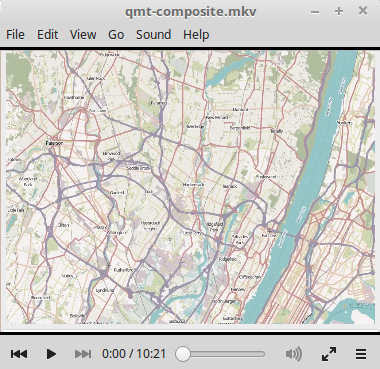
\includegraphics[scale=.4]{pm/qmt-composite.png}\\GIS}}%
 \hspace{10pt}\href{http://www.lingtechsys.com/videos/dhax-composite.mkv}{\parbox{.3\textwidth}{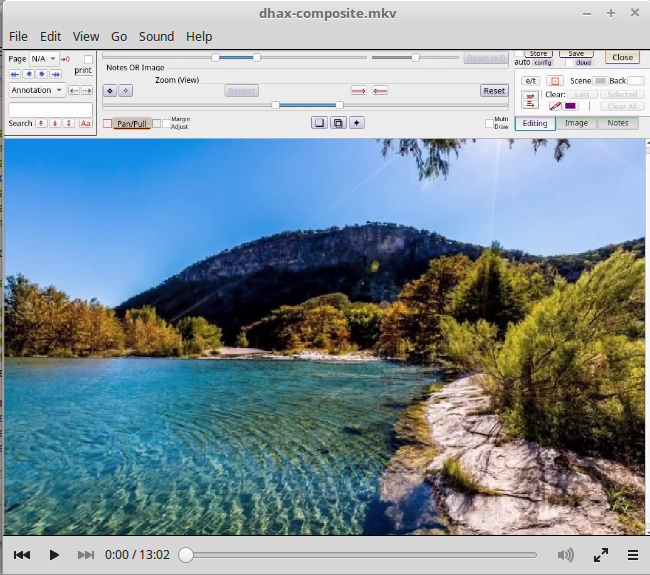
\includegraphics[scale=.255]{pm/dhax-composite.png}\\360\textdegree{} photography}}%
 \hspace{25pt}\href{http://www.lingtechsys.com/videos/xcsd-composite.mkv}{\parbox{.3\textwidth}{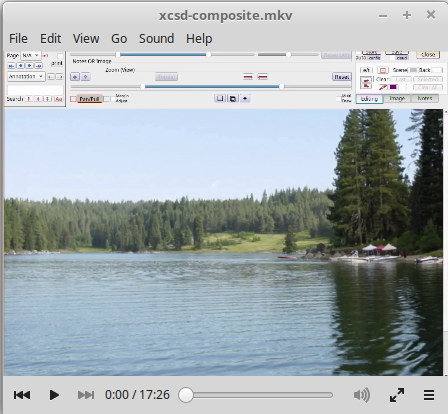
\includegraphics[scale=.35]{pm/xcsd-composite.png}\\Image Processing}}%
}}}\fi
}





%\AddToShipoutPicture*{%
%\ifnum\value{page}=12{
%  \AtPageLowerLeft{%
%    \raisebox{20pt}{%
      
%\hspace*{9pt}\fontsize{11}{11}\selectfont{\textcolor{logoOrange!50!magenta}{%
%\fndiamond{\usepage}}}
%
%    }%
%  }
%\fi}
%}

\definecolor{bkgr}{HTML}{228AFE}

\renewcommand{\descriptionlabel}[1]{\hspace{\labelsep}%
{\fontfamily{lmss}\fontseries{bx}\fontsize{12}{12}\selectfont%
\textcolor{bkgr!50!black}{#1}\hspace*{1.5em}}
}


\begin{document}


%\setlength{\footskip}{22pt}


%\thispagestyle{empty}
\thispagestyle{firstpage}

\vspace*{-76pt}

%\vspace*{1em}

\begin{center}

{\cyanhr}

\vspace*{15pt}

{\color{red!70!black}\fontfamily{phv}\fontseries{b}\selectfont

%\vspace*{13pt}

%{\Large{Solving the Machine Readable Problem}}

%\vspace*{10pt}

%{\Large{by}}

{\large{The Publishing Accelerator Toolkit (PacTk)}}

%\vspace*{7pt}

%{\large{as applied to Multimedia Government, Civil and Environmental Informatics}}

%\vspace*{7pt}

%{\large{Architecture, Construction, and Property Data}}

}

{\cyanhr}

\vspace*{15pt}

\hspace{-32pt}Amy Neustein, Ph.D.\\
\hspace{-32pt}CEO and Founder\\
\hspace{-32pt}Linguistic Technology Systems\\
\hspace{-32pt}Fort Lee, NJ\\
\hspace{-32pt}917-817-2184\\
\hspace{-32pt}\href{mailto://amy.neustein@verizon.net}{amy.neustein@verizon.net}

\end{center}


%{\large{}}

%vspace*{6pt}


%}


\vspace*{1pt}

{\setstretch{1.12}


%\section{Overview}
%\vspace{}
\noindent\subtitle{{Class Libraries and Full-Text Search/Encoding Tools for   \\
\vspace{4pt}
Publishing Documents, Datasets, and Multimedia Resources}}
%\sectvspace{}

\vspace*{2pt}
{\semihr{0.077\textwidth}}
\vspace*{3pt}
%\sectnum{1.}
\hspace{2pt}\secttitle{{Overview}}\sstitletri{7}\sstitletri{2}\sstitletri{2}
\vspace*{5pt}
{\semihr{0.077\textwidth}}

\vspace*{3pt}

\p{In contemporary publishing, the standard workflow includes \XML{}-based 
formats such as \JATS{} or \BITS{}, from which are compiled 
\PDF{}s and other human-visible documents.  Intermediate \XML{} and 
similar files are distinct from those that authors submit directly; 
they have their own tool stacks and 
are computationally accessed via protocols 
such as \SAX{} (Simple \API{} for \XML{}), \XQuery{}, 
\DOM{} (Document Object Model),  
and \XQSE{} (\XQuery{} scripting extension).  Unfortunately, 
\XML{} itself is not explicitly built for representing 
textual data, and examining \JATS{} or \BITS{} files via 
generic \XML{} technology renders certain publishing-related 
query and editing tasks difficult to implement.  The \PDF{} format 
is similarly opaque because internal \PDF{} representations 
of document text include many anomalies due to 
ligatures, hyphenation, font specs, and other layout-related 
discrepancies between \XML{} inputs and user-visible output.  
As a result, internal \PDF{} text only partially corresponds 
to textual content as understood by authors, editors, and human readers.}

\p{Given the limitations of \PDF{} and \XML{} for natural-language 
documents, numerous competing formats have been developed, 
providing potential alternatives or extensions to \XML{}.  These  
include \TEI{} (Text Encoding Initiative), \TagML{} 
(Text-as-Graph Markup Language), \BioC{} (a biomedical text mining 
standard defined by PubMed Central), and Research Object Bundles 
(a Semantic-Web based specification that covers both text and 
data sets).  With a proliferation of different text-encoding standards, 
query and traversal protocols that are developed for one  
format (e.g., \JATS{} and its derivatives) cannot be directly applied 
to others.  For example, the \XML{} parent-child element relationship 
is replaced in \TagML{} with two different containment styles 
(logical and extensional), such that \DOM{} and event-based 
parsers targeted at the simpler \XML{} hierarchy must be reimplemented 
for the \TagML{} system.  Meanwhile, with 
regard to \PDF{}, effective search and text-interaction 
capabilities depend on supplementing this format's internal 
natural-language representation with machine-readable text encoding, 
which might be embedded in \PDF{} files or available as sibling 
assets.  In principle, \XML{} documents could supply such 
content, although current pipelines are not set up to 
share \JATS{}/\BITS{} files (for example) in end-user contexts.}


\p{From the perspective of 
\PacTk{}, text encoding evinces a spectrum of distinct 
\textit{topomorphic regimes} where a proliferation of 
incompatible document structures prohibits the emergence 
of common query, traversal, and metadata formats.  The obvious 
problem is that workflows have to be reconstructed 
for each incompatible document specification.  
In practice, such difficulties have almost certainly 
hindered the adoption of theoretically well-founded 
formats such as \TagML{}.}

\p{The idea behind \PacTk{} is that divergent 
formats cannot be satisfactorily reconciled simply by 
proposing yet another format to insert into 
analogous workflows.  Instead, building a more 
sophisticated publishing platform involves 
constructing integrated computational 
tableaux weaving together text-encoding, 
query-evaluation, compiler-theoretic, and 
front-end concerns.} 

\p{One important variation amongst text-encoding formats is 
the level of granularity for textual elements.  In 
\JATS{}, \BITS{}, and most \JSON{} encodings, the fundamental 
discursive unit is the individual paragraph.  Elements on smaller 
scales (such as sentences or block quotes) are notated 
haphazardly at best.  \LaTeX{} employs reasonable 
sentence-boundary heuristics --- which may be overridden via 
macros when necessary --- but \LaTeX{} sentences are not expressed 
in any systematic manner (e.g., via auxiliary files) for 
any purposes other than visual spacing.  In \TEI{} and \BioC{}, individual 
sentences \textit{can} be represented, but this is not 
mandatory (thus \textbf{s} and \textbf{sentence} tags 
are available but not guaranteed to be present in any particular document).  
By contrast, \PacTk{} is explicitly built around 
sentence-level units, specifically a \q{topomorphic 
sentence-level object model} (\TSOM{}): when all regular 
text in a natural-language document is explicitly 
contextualized in a delineated sentence object, many 
editing, indexing, and user-interface tasks become feasible 
(as outlined in the next section).}

\p{In contrast to the other formats mentioned here, 
\PacTk{} is not a single file type but rather a collection 
of code libraries and classes, with data types representing 
specific textual elements (sentences, paragraphs, \PDF{} pages, 
annotations and comment-boxes, etc.).  Query and traversal 
protocols modeled via \XQuery{}, \DOM{}, and so on become 
expressed by object methods and operators exposed to 
\Cpp{} code, for example (\PacTk{} is thus \q{topomorphic} 
in the sense that navigation between objects is determined 
by structural properties of divergent document formats, 
that manifest in competing notions of individuation for 
structure-sites and any interrelationships declared between them).  
In short, the \PacTk{} object system synthesizes distinct 
structuring protocols found in competing formats such as 
\JATS{}, \TagML{}, and \BioC{}, allowing publishers' workflows 
to encompass each of these formats (and others) without 
sacrificing compatibility.  \lPacTk{} is particularly 
aimed at publishers who feel constrained by the limitations 
of \JATS{} or \BITS{} but are reluctant to try alternatives 
(\TagML{}, \BioC{}, etc.) due to minimal software-ecosystem support 
and the lack of standardized \XQuery{} and \DOM{}-style interfaces.}\clearpage{} 

\vspace*{-2em}
\p{\lPacTk{}'s design also reflects trends in scientific research 
and the emergence of interdisciplinary fields such as 
social ecology, translational medicine, and medical humanities. 
It is the viewpoint of \PacTk{}'s developers that 
the value of new investigations cannot be fully 
expressed in single-disciplinary terms, nor does one individual 
publication mark the end of a well-conceived research 
project.  Instead, publications are milestones in the 
unfolding of projects that, in the best case, 
progress to socially-beneficial deployments.  
More so than in the past, research projects 
(summarized but not fully articulated by 
academic papers) can serve as foundations 
for scholars' and scientists' technical \q{identity,} 
potentially more significant than details such as degree specialization 
or disciplinary affiliation.  In recognition of 
these paradigms, \PacTk{} seeks to help 
authors build multi-faceted presentations 
covering data, code, and foundations for practical 
applications, which authors could build upon 
for future research work, funding, translational 
implementation, and implementational feedback.}  

\p{The remainder of this document will discuss how 
\PacTk{} can streamline editing, indexing, and document-preparation 
tasks, as well as improve User Experience for human readers.  
Later sections will also address how \PacTk{} may contribute 
to broader projects where text documents are published alongside 
data sets and/or multimedia presentations.  Overall, 
\PacTk{} presents a unified model and coding interface for 
text queries operating in diverse contexts, including 
\PDF{} viewers, search engines, document-preparation code, 
and editing/typesetting.
Similarly, software employing \PacTk{} to navigate through 
document objects can leverage interop metadata across multiple 
formats --- such as \XML{} elements and \PDF{} page 
coordinates --- that is typically unavailable in other publishing tools.}


\vspace*{20pt}
{\semihr{0.380\textwidth}}
\vspace*{5pt}
%\sectnum{1.}
\hspace{2pt}\secttitle{{Features for Editing, Indexing, and PDF Viewers}}\sstitletri{7}\sstitletri{2}\sstitletri{2}
\vspace*{5pt}
{\semihr{0.380\textwidth}}

\vspace*{5pt}

  
\p{The computational foundation of \PacTk{} is a collection of 
classes that represented individual sentences and other 
textual elements in the \TSOM{} family (\PDF{} pages, annotations, 
footnotes, block quotes, edits or changes across document versions, etc.).  
In order to initialize these objects, \PacTk{} provides a distinct 
input format called \GTagML{}, or \q{grounded} \TagML{}.  
The term \q{grounded} reflects how certain structure-sites 
may be specifically marked as serializing a typed object: 
i.e., tags, attributes, or text nodes in the neighborhood 
of a site supply the information necessary to initialize an 
object-instance during deserialization.  In other respects 
\GTagML{} follows most of the principles advocated by 
\TagML{}, with novel extensions; for example, \GTagML{} 
encourages the exploitation of Unicode Private Use areas 
to disambiguate visibly similar but logically distinct characters/glyphs 
(e.g., periods may embody punctuation, acronyms, or abbreviations).}


\p{In source files, \GTagML{} is loosely based on Markdown, so 
authors familiar with Markdown from more informal contexts 
(e.g., social media, chat rooms, \GIT{} documentation, etc.) 
will recognize many of the \GTagML{} styling commands.  
\lGTagML{} sources might be provided by authors directly, or 
derived from author inputs by digital copy editors or 
others on the manuscript pipeline.  To support 
\GTagML{}, \PacTk{} provides a new \Cpp{} parsing library 
that is readily extensible (more so than parsers for 
\XML{}, \JSON{}, and so forth), allowing publishers to 
customize the \GTagML{} format with new tags, syntax, and 
data structures specific to their in-house styles and 
disciplinary focus areas (e.g., specialized tags/data for 
different scientific fields --- chemistry, physics, medicine, 
etc.; or whatever subject areas are addressed by given 
publishers, journals, and book series).  Alternatively, 
\TSOM{} objects could be compiled from sources such as 
\JATS{} or \BITS{} directly.}

\p{For workflows that feature \JATS{}, \BITS{}, or 
\LaTeX{}, \TSOM{} objects may be employed as 
adjunct data sources through which edits, queries, 
document version-comparisons, 
and other computational artifacts are routed.  
\lPacTk{} data can then be mapped both to 
archiving formats (like \XML{}) and camera-ready 
generators (like \LaTeX{}), but with a common 
\TSOM{} background these two different representational 
facets may be integrated (for example, \XML{} elements 
mapped to corresponding \PDF{} page coordinates).  
In effect, \PacTk{} serves to triangulate human-visible 
presentations (like \PDF{}) with behind-the-scenes 
\JATS{}-style formats.  Analyses that are currently 
implemented against \XML{} structures may be more 
efficiently coded via \PacTk{} objects, with concrete 
benefits in areas such as copy-editing and indexing.}



\begin{figure}[ht]
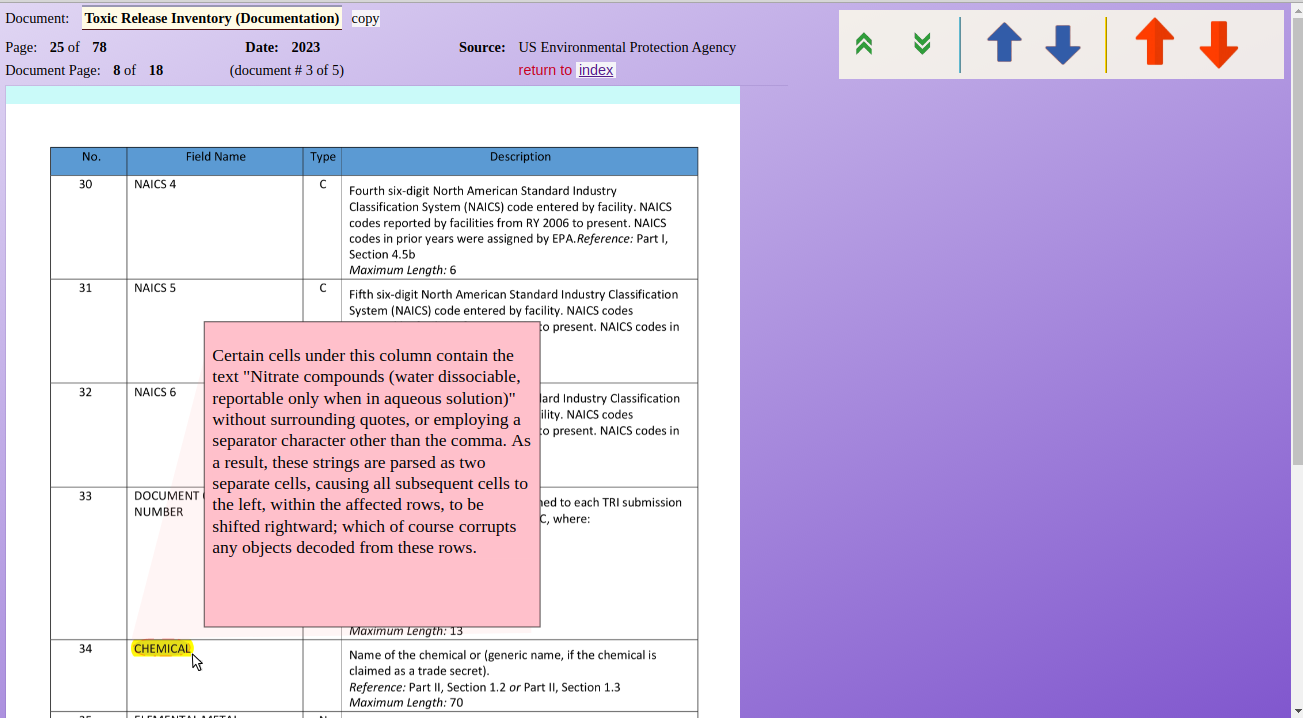
\includegraphics[scale=0.8, trim=0 18pt 0 0, clip]{fin/tox.png}
\caption{Mapping PDF pages to SVG views for improved annotation support}
\label{fig:ss1}
\end{figure}


\vspace*{-2pt}

\sstitle{PacTk for Editing}

\vspace*{8pt}

\p{\lPacTk{} has an advanced query framework to help find 
specific locations in text where edits might be warranted 
(e.g., to comport with journal or book-series conventions) and 
to correctly review and process such edits.  Here are some features:

\begin{description}

\item[Contextual Filters for Text Locations]  Often it is 
useful to restrict the scope of text searches to 
content with specific presentation characteristics (italics, alternative 
typefaces, citations), discursive roles (inline/block quotes, 
footnote text, section/subsection titles), or semantic 
significance (acronyms, annotations, proper/place names).  

\pseudoIndent{} Implementing such filters via \XPath{}/tag 
restrictions can be inaccurate, because relevant filter 
criteria could be orthogonal to \DOM{} hierarchies.  For 
example, \XML{} or \LaTeX{} code might wish to wrap 
elements such as footnotes or block quotes in 
custom environments, to ensure desired pre- or 
post-processing.  Material that is functionally 
footnote or quoted text, therefore, may not necessarily 
be indicated with those specific tag names.  The \PacTk{} 
system allows programmers to define lists of boolean 
parameters that apply to text-sequences and then 
activate those flags automatically in specific tag contexts.



\pseudoIndent{} In general, \PacTk{} supports queries where ordinary 
textual restrictions may be augmented with filters 
for a wide variety of layout and discursive contexts.  
Such queries could then be used for editing 
tasks that should be localized to specific contexts, 
or where a user wants to find a specific piece of 
text known to have a given context.


\item[Sentence-Level Queries]  Siting queries relative 
to sentence boundaries can improve 
precision and express query rationales more succinctly 
(when compared to paragraph-based organization).
For instance, the proper punctuation around a word or 
phrase often depends on whether that content appears 
at the beginning, middle, or end of a sentence.  
Some query expressions might similarly depend on 
stipulating that two or more search targets 
(e.g., two proper names) occur in the same sentence.

\pseudoIndent{} Because \PacTk{} recognizes almost all text as 
contained inside sentence objects, queries dependent 
on sentence boundaries can be directly 
evaluated on \TSOM{} data (such boundaries are 
unambiguously notated via input sources, rather 
than detected approximatively using Natural Language 
Processing).  \lPacTk{} likewise models 
\q{topomorphic} navigational 
relations between sentences, such as between 
adjacent siblings of parent objects (typically 
paragraphs) and also nestings wherein a multi-sentence 
footnote, for example, occurs in a parent-sentence 
context, or where a block quotes functions in part as a 
logical child of the sentence that introduces it.

\item[PDF Page Coordinates]  Human readers post-publication 
--- plus authors and copy editors beforehand --- typically 
view documents in \PDF{} format for normal reading, even if 
edits/changes are made on intermediary files.  As a result, 
a bitmapped page-image is the primary medium through 
which users view single publication pages.  Such graphics are 
typically rendered by \PDF{} viewers, but other 
techniques might be used, such as converting page images 
to \SVG{} (illustrated here in Figure~\ref{fig:ss1}, 
where the relevant component is an embedded web engine 
that communicates with a \PDF{} viewer by 
\textbf{QWebChannel}; so \SVG{} events are 
processed by \Cpp{} code directly, having only a 
minimal \JavaScript{} routing layer).  Failure to 
interoperate these images with structured text formats 
is a significant hindrance to efficient document 
preparation and editing.

\begin{figure}[ht]
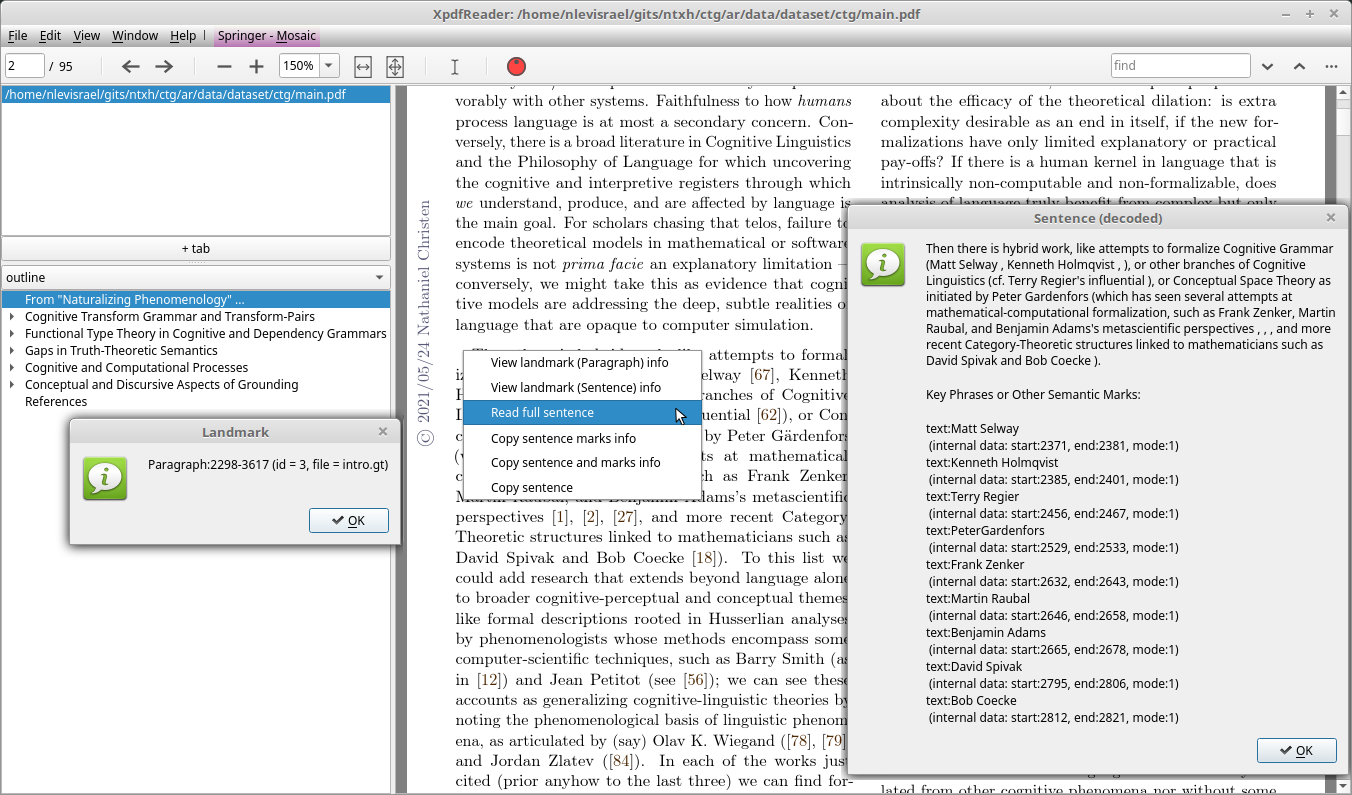
\includegraphics[scale=0.45]{fin/ling.png}
\caption{Enhanced GUI capabilities enabled by machine-readable text encoding}
\label{fig:ss2}
\end{figure}


%\begin{figure}[h!]
%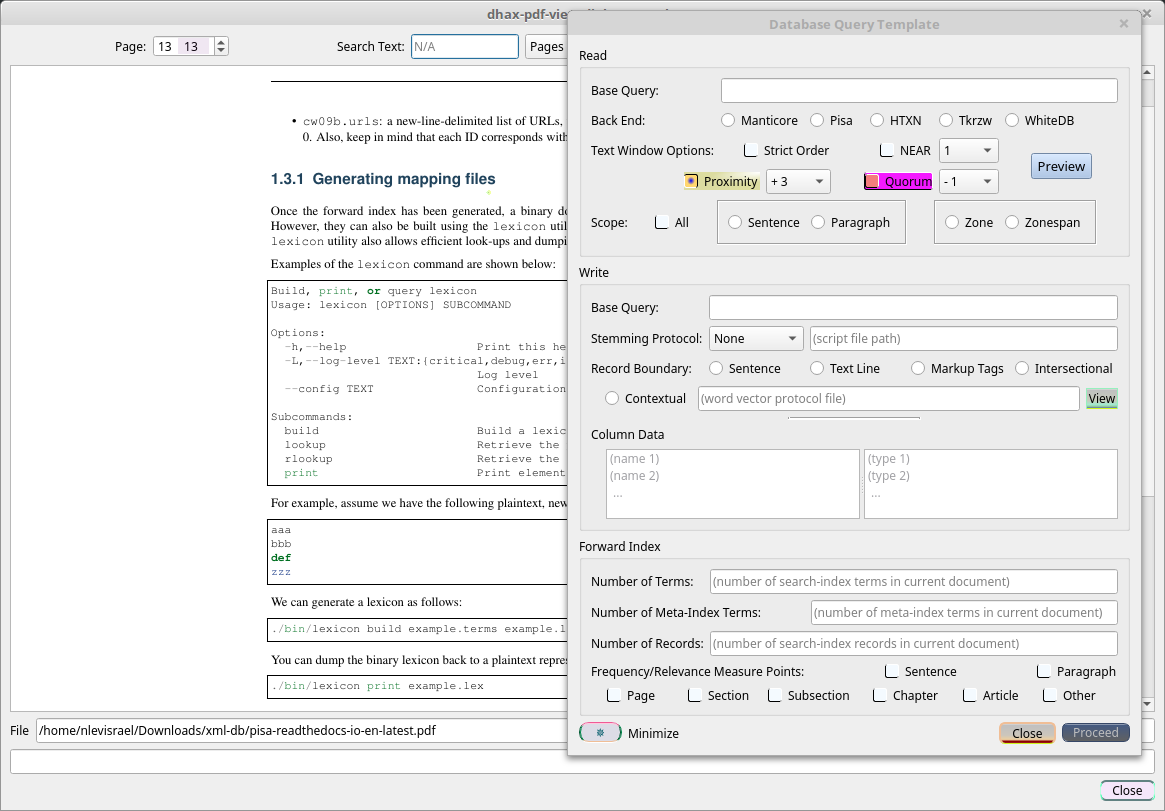
\includegraphics[scale=0.66, trim=8.4cm 0 0 0, clip]{fin/pisa.png}
%\caption{Configuring Default Back-End Queries}
%\label{fig:ss9}
%\end{figure}

\pseudoIndent{} By design, \PacTk{} supports post-processing 
algorithms within pipelines whose formats can generate 
\PDF{}-coordinate metadata, such as \LaTeX{} 
\textbf{pgfsavepos} (and auxiliary \textbf{write}) commands.  
Page coordinates for significant discursive locations 
(e.g., sentence and paragraph boundaries, footnote markers, 
keyphrases and named entities, citations) can thereby be 
exposed to \PDF{} viewers which could accordingly implement 
novel front-end features such as overlays, context menus, 
and dialog windows positioned nearby relevant content 
(Figure~\ref{fig:ss2}).  
For example, a context menu action may include copying the 
full text of a current sentence to clipboard, based on the 
screen position where the menu is activated; semitransparent 
overlays could similarly show the extent of individual 
sentences during mouseover events.
  
\item[PDF Comments and Annotations]  In addition to sentence 
objects, \PacTk{} classes model data specifically relevant to 
the \PDF{} front-end milieu, including single pages, links/anchors, and 
comments/annotations.  Objects such as comment-boxes 
may thereby be leveraged systematically in an editing/review pipeline.

\pseudoIndent{} In particular, \PacTk{} supports construction of hashtag- or handle-style 
controlled vocabularies that could annotate \PDF{} comments 
introduced by copy editors or typesetters.  Many modifications considered 
during the editing process follow common patterns, such as 
proper use of commas around subordinate clauses, or correct formatting 
of ellipses and bracketed content within inline/block quotes.  Assuming 
that editors consistently include notations for recurring patterns, 
\PacTk{} code can filter queries specifically to \PDF{} comment 
boxes which indicate a specific editing category.  Index codes within 
\PDF{} comments may likewise indicate which individual sentence 
surrounds the annotation, so that the \PDF{} view could be cross-referenced 
against input sources, which facilitates review and processing 
of manuscript changes.


\pseudoIndent{} For similar reasons, \PacTk{} supports abstractions 
such as \XML{} custom character entities and \LaTeX{} macros.  
Many familiar textual components --- ellipses, 
\textit{m-} and \textit{n-}dashes, 
quotation and footnote marks, etc. --- are typically represented 
not via their visible characters but rather through standardized 
codes or glyphs.  The problem is that systematic mappings 
are lacking when mixing different file types (e.g., \LaTeX{} and 
\XML{}, such as \JATS{} or \BITS{}) in a single workflow.  
\lPacTk{} has a flexible abstraction system that allows 
character and macro codes to propagate across different 
generated files.


\pseudoIndent{} A related problem is that abstraction codes should 
generally be opaque to human users in contexts such as 
comment boxes and copy-paste between software applications.  
\lPacTk{} therefore supports declarations for how 
custom entities/macros and Unicode Private Use Plane 
(or area) codepoints 
should be rendered in plain-text contexts as well as 
structured formats such as \XML{} and \LaTeX{}.        
 
\end{description}
}


%\begin{figure}[ht]
%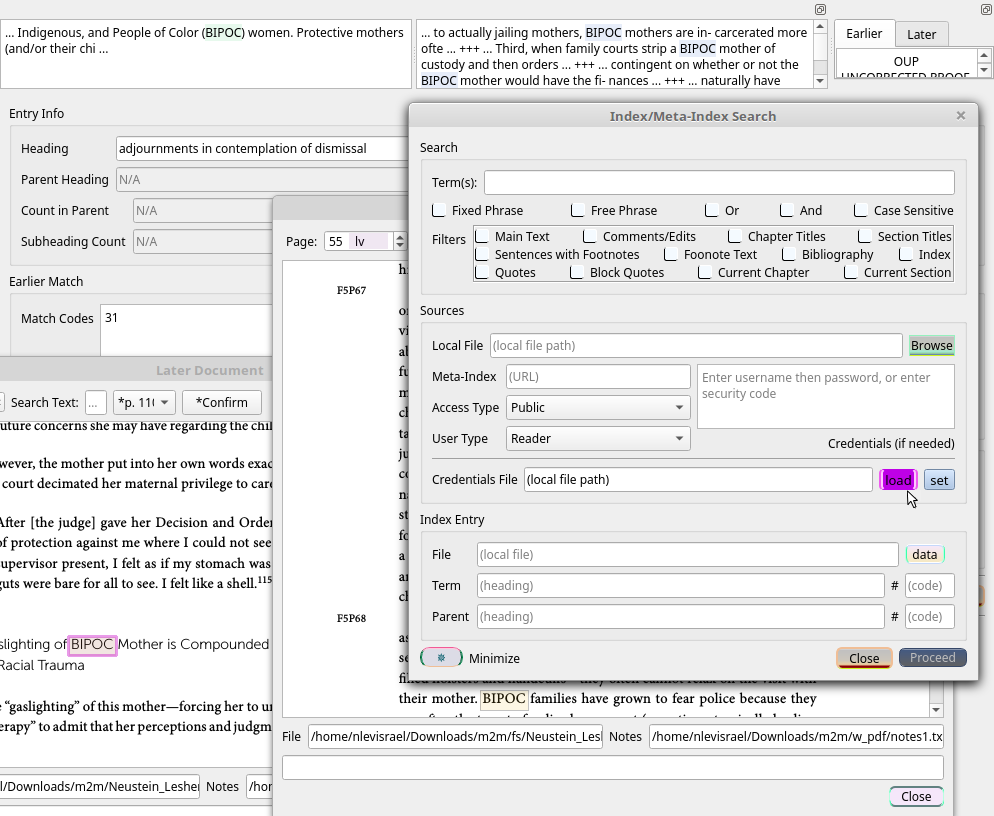
\includegraphics[scale=0.83]{fin/meta.png}
%\caption{Dialog window for local and meta-index searches}
%\label{fig:ss2}
%\end{figure}

\vspace{-.85em}\enlargethispage{.5em}

\p{Often users may prefer to initiate or review edits through \PDF{} files 
directly, but in other cases plain-text files might be appropriate 
instead, without \GUI{} overhead.  With \PacTk{}, for example, 
authors could receive a pair of text files (or collections of files 
indexed, for instance, by chapter) summarizing changes between 
two manuscript versions.  Via sentence-level filtering, 
such files could be organized such that only sentences that 
differ from one version to the next are included, with each 
sentence listed separately.  This may be a more convenient 
setup for authors to review changes than working through 
typical \GUI{}s (structured text encoding is 
important because it ensures that version comparisons 
show valid differences, rather than anomalies 
due to inconsistent characters and symbolization).
Of course, such breakdown is only possible 
when the text encoding systematically identifies individual 
sentences, as with \PacTk{}'s \TSOM{} object model.}

\begin{figure}[b!]
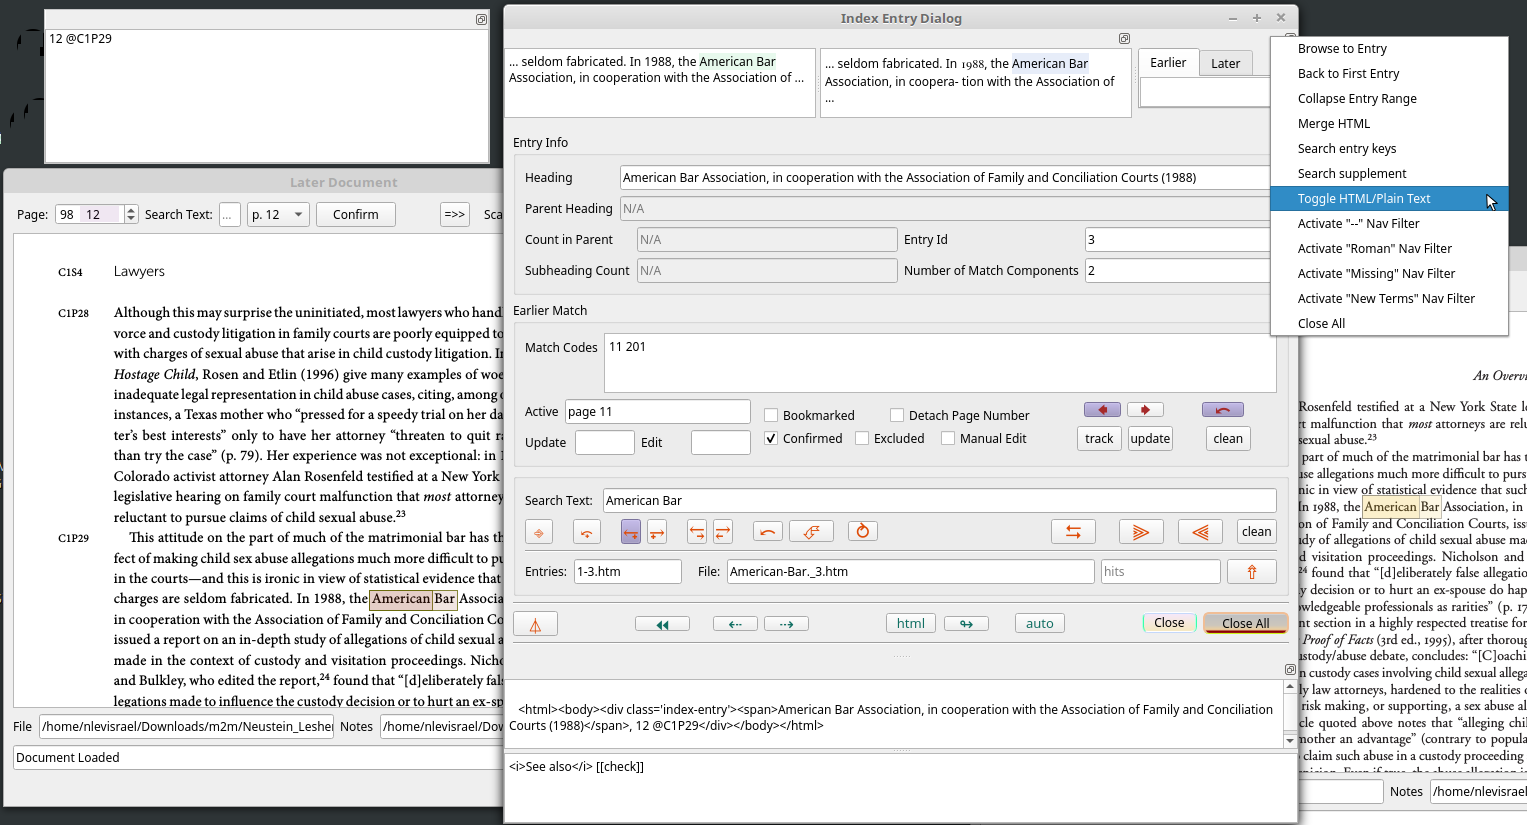
\includegraphics[scale=0.4]{fin/ie.png}
\caption{GUI functionality for compiling and curating indexes}
\label{fig:ss3}
\end{figure}



\begin{figure}[t]
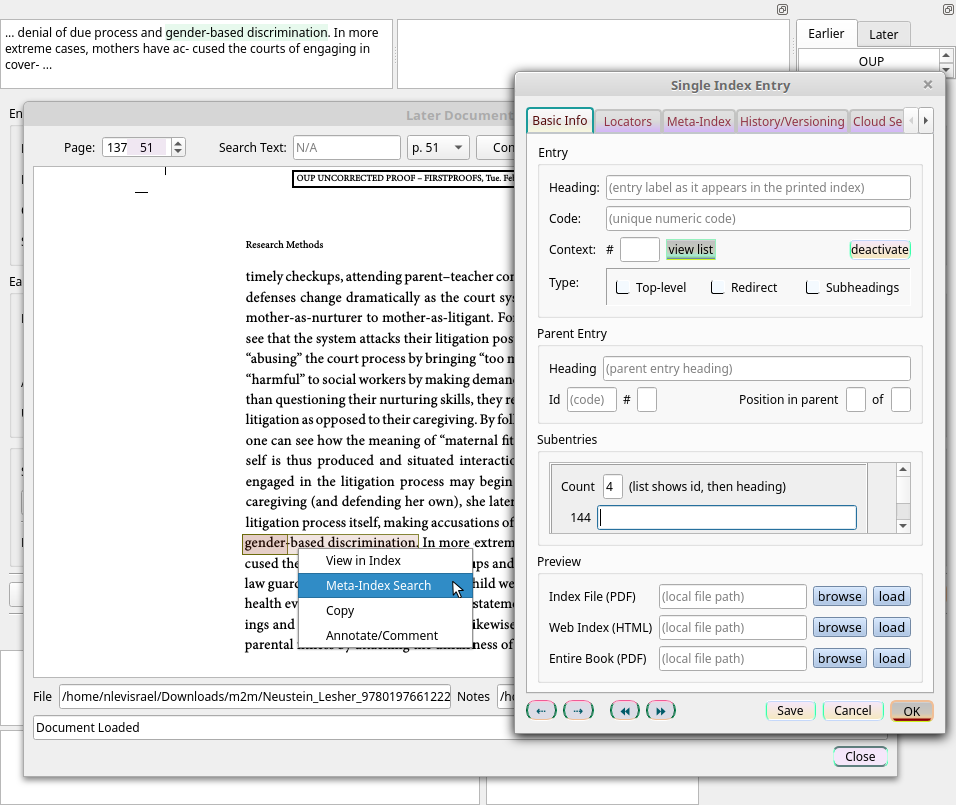
\includegraphics[scale=0.83, trim=0 4.1cm 0 0, clip]{fin/single.png}
\caption{An index entry dialog window (and context menu for single and meta-index views)}
\label{fig:ss4}
\end{figure}


\vspace*{4pt}
%{\semihr{0.31\textwidth}}
%\vspace*{5pt}
%%\sectnum{1.}
%\hspace{2pt}\secttitle{{PacTk for Indexing and Search Engines}}
%\vspace*{5pt}
%{\semihr{0.31\textwidth}}

\sstitle{PacTk for Indexing and Search Engines}


\vspace*{7pt}

\p{Authors might use one of several methods to compile an index.  
They can start with a list of important headings 
(names, concepts, etc.) and search for relevant passages in the 
manuscript.  Alternatively, authors could read through a 
document and identify when a particular paragraph mentions a 
named entity suitable for indexing.  Depending 
on representations or tag sets used (e.g., the 
\JATS{} \textbf{string-name} element) annotated spans 
and citations may also form the provisional heading-list 
for an index.}


\p{Given these various index-preparation methods, it is useful to 
extend front-end tools with capabilities specific to indexing 
workflows, such as query matching and manipulating index entry objects.  
Structured formats like \JATS{} do not provide sufficient 
computational tractability in themselves.  For example, the most 
popular desktop \GUI{} framework are the \Qt{} \Cpp{} libraries, 
which are the basis of cross-platform \PDF{} viewers such as 
Poppler and \XPDF{}.  \lPacTk{} can seamlessly interoperate 
with \Qt{}, exposing sentence texts as \textbf{QString} objects and 
expressing \GTagML{} parsing grammars as \textbf{QRegularExpression} 
instances, paired with lambda callbacks activated by the first matching 
rule (relative to the current parse-position).  More precisely, 
\GTagML{} has context-sensitive grammars that can include or 
skip over rule-tests via activated contexts; this allows sections 
of a \GTagML{} file to utilize syntax different from the default.}

\p{With respect to indexing, \GTagML{} has its own notation for 
index entries (headings, locators, and \q{see also} style redirections), 
to serialize indexes in a human-readable format.  Correspondingly, 
\PacTk{} has classes specifically for index entries and 
associated data.  These objects could be initialized from 
\GTagML{} files or specialized windows floating atop 
\PDF{} viewers.}



\p{Building indexes on the basis of native sentence and index-entry objects 
has certain benefits as compared to generic (e.g., \XML{}) manuscript 
formats.  These include:

\begin{description}

\item[Multiple Match Strategies]  Index locators are typically 
identified by matching text against entry-headings, but the parameters 
of these searches will vary by context.  Sometimes locators are 
only relevant when the local sentence includes just the exact 
heading label, but in other places a desired match could 
include words in different order (e.g., either first-name/last-name 
or vice-versa), or a subset (e.g., last name only), 
or associated concepts with different language entirely 
(e.g., \q{The White House} in lieu of a president's name). 
Concepts can also be grouped into semantic \q{clusters} 
(consider \textit{ranson}, \textit{extortion}, \textit{bribery}, 
\textit{corruption}, \textit{influence peddling}, \textit{lobbying}), 
with internal similarity-weight matrices.  In the 
presence of a particular index entry, front-end displays can 
give users options to fine-tune which match strategies are 
appropriate for query strings seeking locators specific to that entry.



\item[Separating Data from Presentation]  Different publishers 
or book series may choose different visual styles for their 
indexes.  Representing indexes behind the scenes via structured 
data objects allows them to be curated in abstraction from the 
specific layout chosen for final publication.  

\vspace{-3pt}

\item[PDF Context Menus]  Authors/editors may prefer to add new index entries 
or locators directly from \PDF{} pages.  \lPacTk{}-compliant 
viewers will read metadata that specifies which paragraphs are 
in scope at different page-coordinate regions, so paragraph ids 
for any location can be ascertained from mouse events (e.g., 
the dropdown point of a context menu).

\vspace{-3pt}

\item[Index-Building GUI Components]  Index entries are multi-faceted 
objects that naturally lend themselves to dedicated front-end displays, 
such as dialog windows (Figures~\ref{fig:ss3}~and~\ref{fig:ss4}).  
For example, entries typically include a heading 
label and then one or more locators (e.g., paragraph ids, replaced 
eventually with page numbers), 
then possible subheadings with their own 
locators, plus \q{redirectors} (\textit{see} or \textit{see also}) applied 
either to overall entries or to subheadings.  This represents a lot 
of information to keep track of for each entry, and indexes can include 
hundreds of entries.  Although indexes are eventually shown 
to readers as ordinary \PDF{} pages (or similar formats), 
during document prep it is useful to subdivide indexes into 
individual \GUI{} windows for each entry, with options to 
navigate between adjacent entries or to traverse on larger 
scales (e.g., one chapter to another), plus to create new 
entries on the fly.

\vspace{-3pt}

\item[Index-Guided Text Searching]  Indexes are curated lists 
of headings and locators selected by authors/editors for 
relevance.  Whenever a search is posed against a manuscript in 
any context --- e.g., in the query bar of a \PDF{} viewer, or 
an online search engine, or \XQuery{}-style terms evaluated 
\visavis{} \JATS{} files --- index metadata can be consulted 
just in case search terms overlap with headings already included 
in an index.  Such functionality may be augmented by extending 
index metadata to include concepts related to index entries 
even if those secondary concepts are not indexed themselves 
(as with semantic clusters, mentioned above).
In effect, index metadata may declare that all locators 
modeled as relevant for their specific entry are also relevant 
to some list of associated concepts, such that whenever those 
latter concepts are targeted in a query the explicit 
locators are included among the query results (Figure~\ref{fig:m2m}).   

\vspace{-3pt}

\item[Series or Archival Meta-Indexes]  Once a standard format 
is developed for indexes in some document collection, it becomes 
possible to pool multiple instances into a common archive.  
Each time a new publication is finalized, all of its index 
terms could be inserted into a bibliographic database 
allowing users to search across multiple books/manuscripts 
in a given book series, journal %{\textcolor{white}X}\vspace*{2pt}
%\textcolor{white}{collection, or document repository.  Such meta-indexes can support searches that are more precise and granular than conventional}
collection, or document repository.  Such meta-indexes can support searches 
that are more precise and granular than conventional
search-engine technologies based on occurrence vectors 
and stemming/lemmatization alone (Figure~\ref{fig:ss5}).\clearpage

%\vspace*{-2pt}{\tiny XXXXXXX}


\begin{figure}[h!]
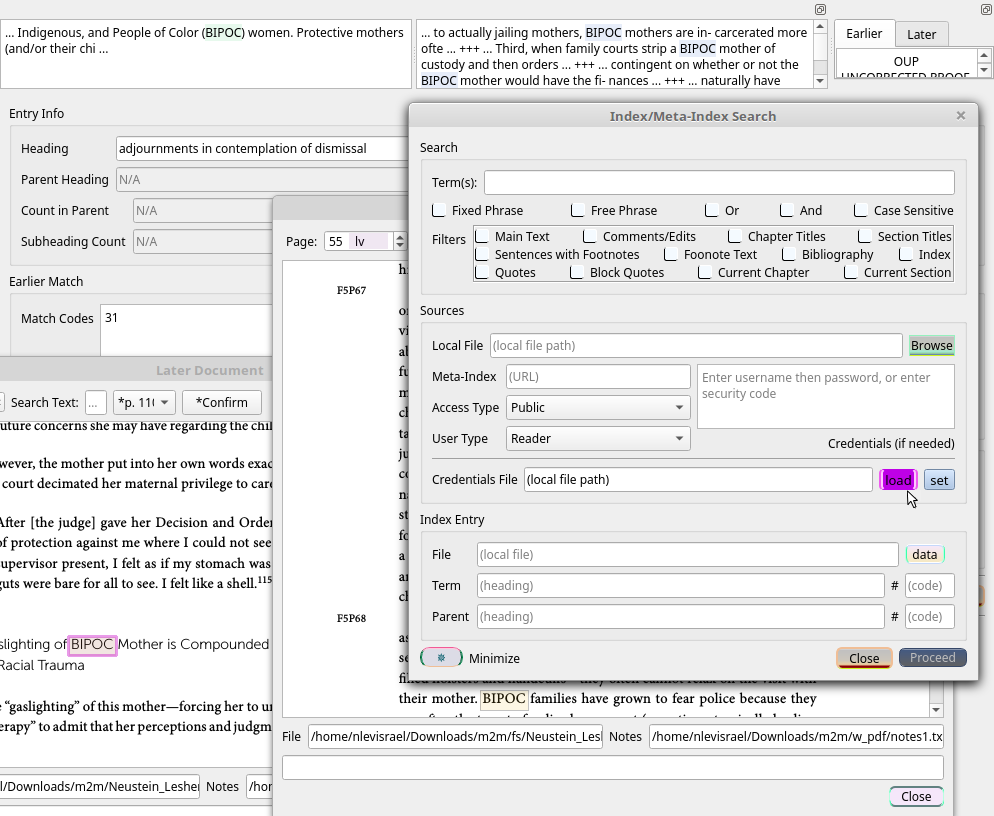
\includegraphics[scale=0.83]{fin/meta.png}
\caption{Dialog window for local and meta-index searches}
\label{fig:ss5}
\end{figure}


\par\noindent\vspace*{-24.5pt}%\textcolor{red}{\rule{\textwidth}{0.4pt}}
\enlargethispage{4em}

\item[Academic Search Engines]  In online contexts, \q{indexing} typically 
refers not to human-visible book indexes but rather to 
compressed data files that catalog nontrivial words 
and concepts in a manuscript.  Such indexing is typically 
non-contextual; for example, it is not represented whether a 
word/phrase is present in text with a special purpose 
(quotes, footnotes, chapter/section titles, etc.) and 
sentiment/discursive roles are ignored (e.g., a document might be identified as 
\textit{about} some topic, but more specific criteria 
such as arguing \textit{for}, \textit{against}, or neutrally 
\textit{evaluating} theories or claims are not modeled).  
Granularity may be limited by the scope of an archive, because 
efficient queries can only expend a few seconds per 
document if searches are to be conducted against a large collection.  

\pseudoIndent{} Nevertheless, search functionality can take 
steps to increase query specificity via meta-indexes and 
related metadata.  For one thing, users may specifically 
consult search areas that are restricted in scope --- say, a single 
University Press, book series, repository (PubMed Central, for example), 
or journal collection.  Publishers who curate meta-indexes 
for mid-size collections can support much more detailed 
evaluations per document; a book series might have several 
dozen titles, not tens of thousands.  \lPacTk{} supports 
construction of corpora query languages that express 
granular searches over multiple documents, with 
similar logic to filtered/contextualized text searches 
in a single \PDF{} document (Figures~\ref{fig:ss6}~and~\ref{fig:ss7}).
Even where queries are executed via conventional 
vector-database methods, \PacTk{} allows authors or digital editors 
to exercise control over how word-occurrence lists are compiled.  
For example, \TSOM{} objects can include lemmatized word-lists 
per sentence; authors may then control for 
circumstances such as two different meanings reduced to the 
same linguistic stem, which might not be properly 
ingested by search engines indexing documents 
through their default algorithms.

\pseudoIndent{} Although \lPacTk{}'s originating focus is publishing 
--- where the primary components of a repository are 
manuscripts/documents in formats like \PDF{} --- this technology 
could potentially be used in other environments.  For instance, 
in clinical trials and point-of-care software the fundamental assets 
are Electronic Health Records; but search features, 
as well as plugins and multimedia (discussed next),
might be extended to include resources such as diagnostic 
images, cytometry gating, assay graphics, 
tumorogenesis simulations, etc.  Publishing-related plugin architecture 
(e.g., document viewers in scientific software) may be 
adapted and resued for these \EHR{} contexts.\clearpage

\begin{figure}[h!]
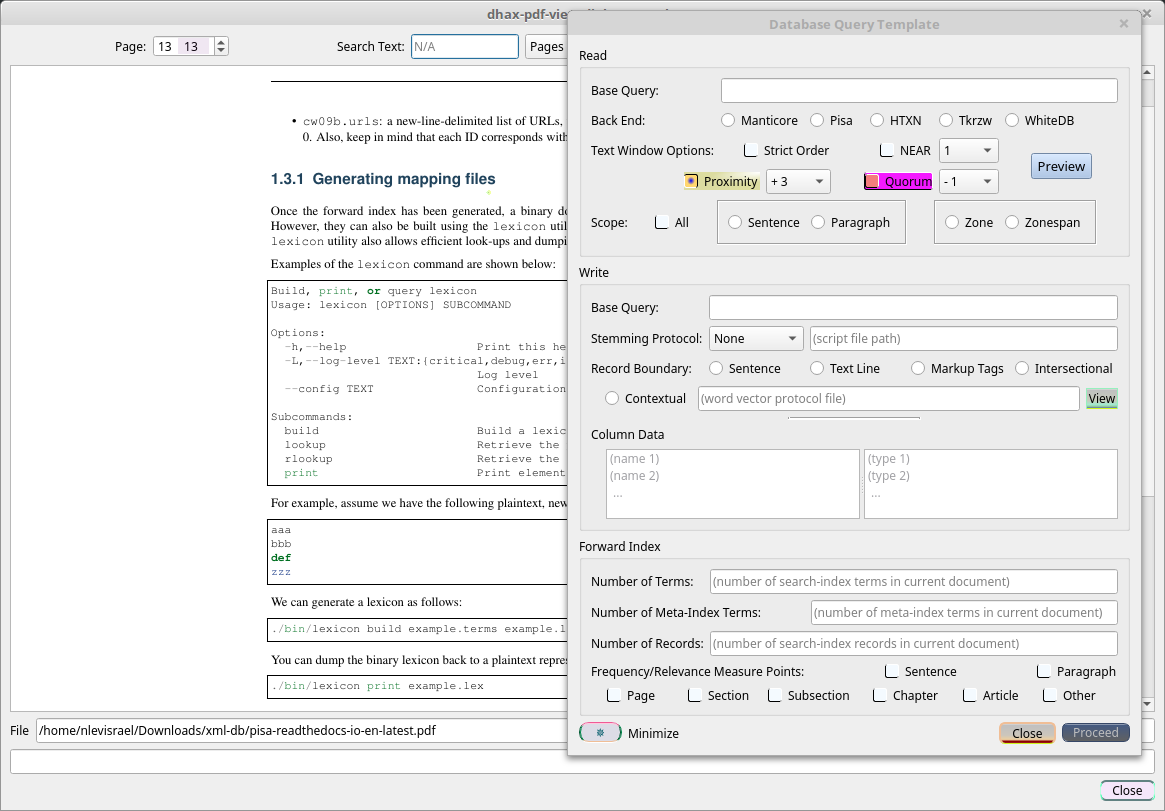
\includegraphics[scale=0.66, trim=8.4cm 0 0 1cm, clip]{fin/pisa.png}
\caption{Configuring default back-end queries}
\label{fig:ss6}
\end{figure}

%\begin{figure}[h!]
%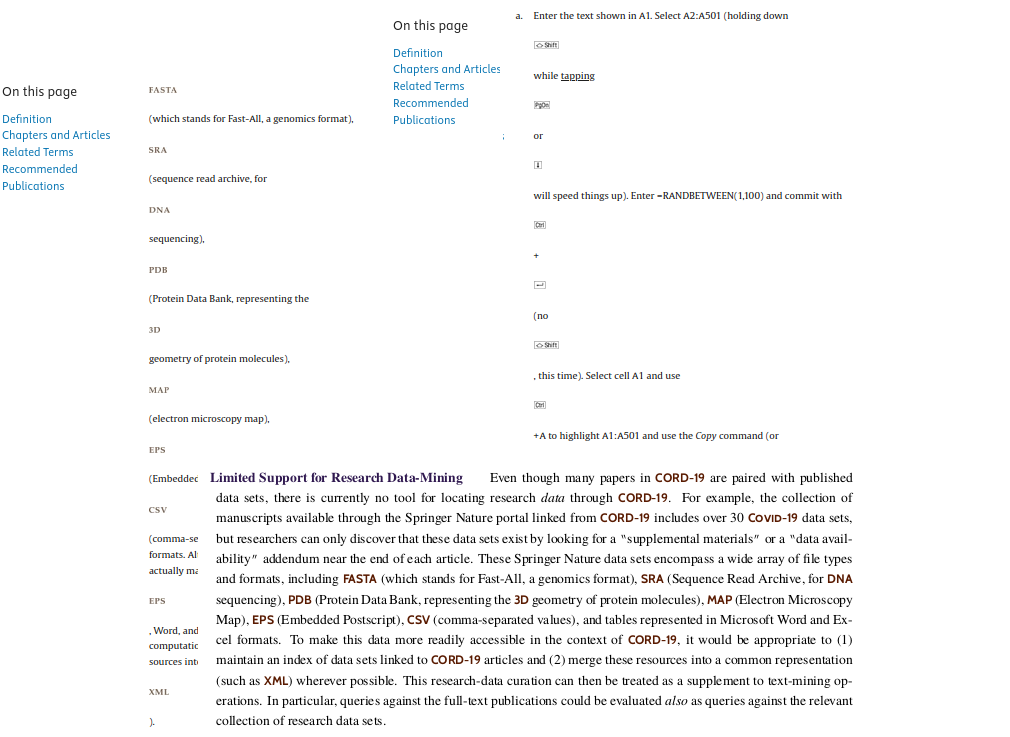
\includegraphics[scale=0.71, trim=0 0 0 0, clip]{x/x2.png}
%\caption{HTML Transcription Errors}
%\label{fig:ss6a}
%\end{figure}

\item[Accurate Search Portals]  For users accessing search functionality 
through online \HTML{} portals, extra programming is necessary to 
properly show results derived from \PDF{} documents.  Figure \ref{fig:ss10} 
(last page)  
shows two excerpts taken from publications included among 
one publisher's lists of subconcepts under the \q{engineering} heading.  
Both examples show irregular line spacing and improper rendering 
of text with distinct font-styles.  It is clear that the 
intermediate files, from which \PDF{} was produced as expected, 
were less successful in the context of \HTML{} generation 
(an accurate \PDF{} is displayed at the graphics bottom).  
These pages show a weakness in \JATS{}-style encodings 
that can be alleviated by a sentence-object model where 
styling objects have both \LaTeX{} and \HTML{} output content.     

\pseudoIndent{} Another source of transcription errors is 
character strings which are not ordinary language and therefore 
require special encoding rules.  The book on the 
left in the Figure \ref{fig:ss10}\footnote{\hspace*{4pt}Amy Neustein 
and Nathaniel Christen, \textit{Innovative Data Integration and Conceptual Space Modeling for COVID, Cancer, and Cardiac Care} 
(Elsevier, 2022).} was a survey of biomedical software engineering in
several domains, including text mining, radiomics, and immuno-oncology.  
Vis-\`a-vis text mining, the book reviewed \CORDNineteen{}, a 
large open-access document repository curated by the Allen Institute 
for \AI{} (\AItwo{}) to spearhead Coronavirus research.  This corpus, unfortunately 
(and as acknowledged by \AItwo{}) had inconsistent (\PDF{}-based) text 
extraction; e.g., in the aforementioned analysis the authors gave examples of a 
chemical formula that was printed in different styles in distinct 
publications reproduced within \CORDNineteen{}, which could cause the 
overlap on that common semantic element to go unrecognized by 
text mining algorithms.  In response to problems both with 
special-purpose and ordinary text representation, \AItwo{} issued a 
\q{call to arms} encouraging publishers to adopt standardized 
machine-readable encodings as supplements to their \PDF{} (and 
\HTML{}) outputs: \q{Existing schemas like [\JATS{}] can be too coarse-grained to
capture all ...\hspace{3pt}metadata elements, [and]
representations ...\hspace{1pt}vary greatly across 
publishers who use them. To
improve metadata coherence across sources, the
community must define and agree upon an 
appropriate standard of representation}\footnote{\hspace*{5pt}Lucy Lu Wang, \textit{et al.}, 
\q{CORD-19: The COVID-19 Open Research Dataset,} Allen Institute for AI, 2020. 
\href{https://aclanthology.org/2020.nlpcovid19-acl.1.pdf}{https://aclanthology.org/2020.nlpcovid19-acl.1.pdf}}  \lPacTk{} is an example of technology 
that could satisfy these goals. 

\clearpage{}

%\begin{figure}[h!]
%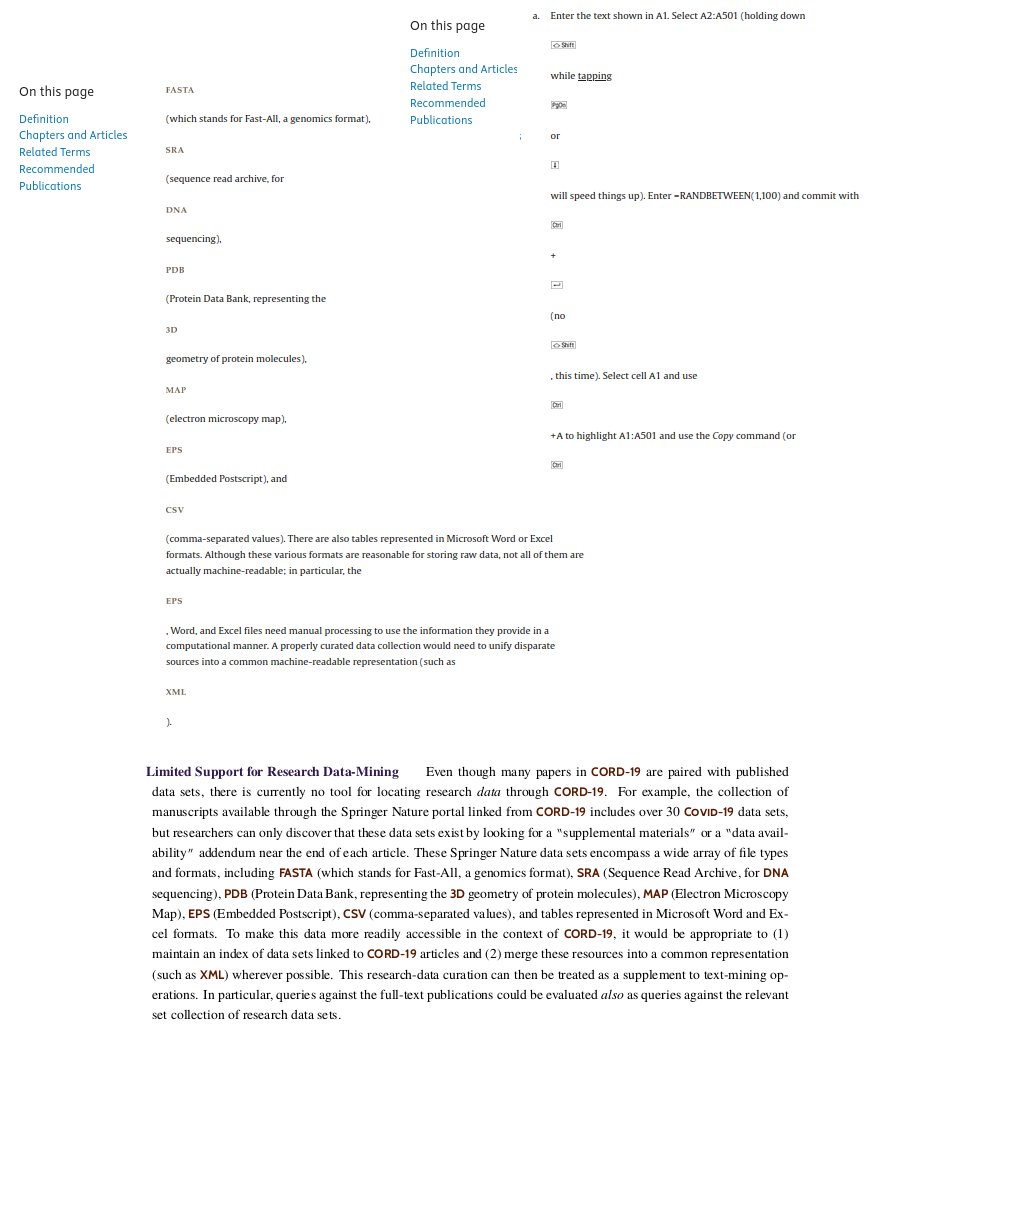
\includegraphics[scale=0.71, trim=0 7cm 0 0, clip]{x/x3.png}
%\caption{HTML Transcription Errors}
%\label{fig:ss6a}
%\end{figure}

%\begin{figure}[h!]
%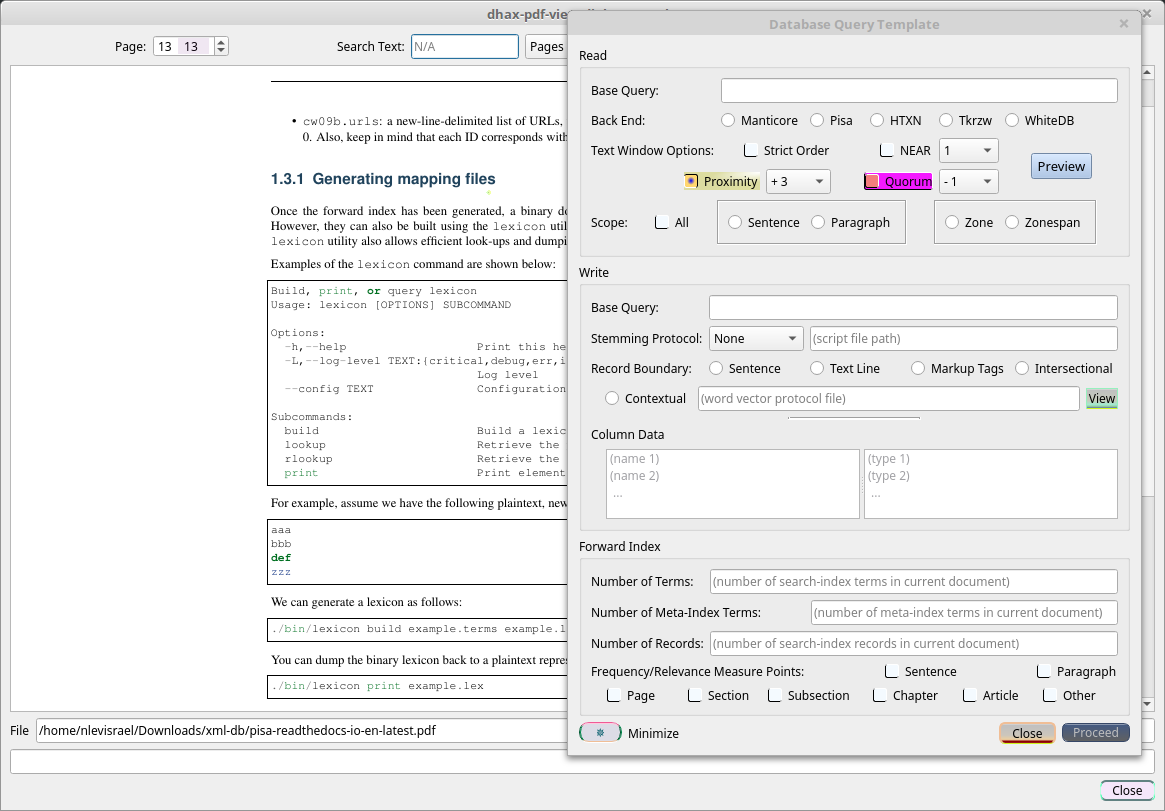
\includegraphics[scale=0.66, trim=8.4cm 0 0 0, clip]{fin/pisa.png}
%\caption{Configuring default back-end queries}
%\label{fig:ss6}
%\end{figure}

\item[Granular Locators]  Current indexing 
tools are migrating to paragraph ids (rather than page numbers) 
for index preparation, although numeric locators still appear 
in the human-visible digital (and, of course, printed) versions.  
For best accuracy, it is worthwhile to partition paragraphs 
that contain block quotes, enumerations, or other subdivisions 
and assign unique ids to each part (see Figure~\ref{fig:xNC}).  
For example, segments of text before and after a block quote 
(plus the quote itself) can have distinct ids, even if they 
are part of the same larger, encompassing paragraph.

\pseudoIndent{} Given this precision, digital indexes even in \PDF{} documents 
can benefit from paragraph ids.  The right-hand part of 
Figure~\ref{fig:xNC} shows an index with color-coding to 
indicate such details as subdivisions (e.g., block quotes) 
and paragraphs split between two pages.  In the 
depicted document, all locators are clickable and 
scroll to a precise location (top of paragraph or of page).

\item[Bidirectional Indexes and Text Extraction]  Assuming index 
entries are pooled into an archival data structure, each entry 
is a potential cross-reference point between multiple documents.  
The concept of a \q{locator} may thereby extend beyond a single 
publication; from any one digital index users could initiate 
searches for matching entries in other books or articles.

\pseudoIndent{} To support such functionality, text encoding should describe 
structured objects (such as \textbf{date} and \textbf{string-name} tags in 
\JATS{}) wherever segments follow canonical encodings beyond 
just natural language (e.g., citations, references, bibliographic 
entries, and quoting/transcription conventions).  Also, via \PacTk{} 
meta-indexes can enforce consistent encoding for special characters 
(e.g., quote marks) and structured segments (e.g., proper-name initials) 
in cases where different style guides have inconsistent recommendations 
(for example, whether or not to include spaces between consecutive initials).  
Treating such portions of a document as unstructured text content 
can obscure cross-references and potential micro-citations, 
as well as cause errors within manuscripts internally. 

\enlargethispage{4em}
     
\begin{figure}[h!]
\hspace{-5em}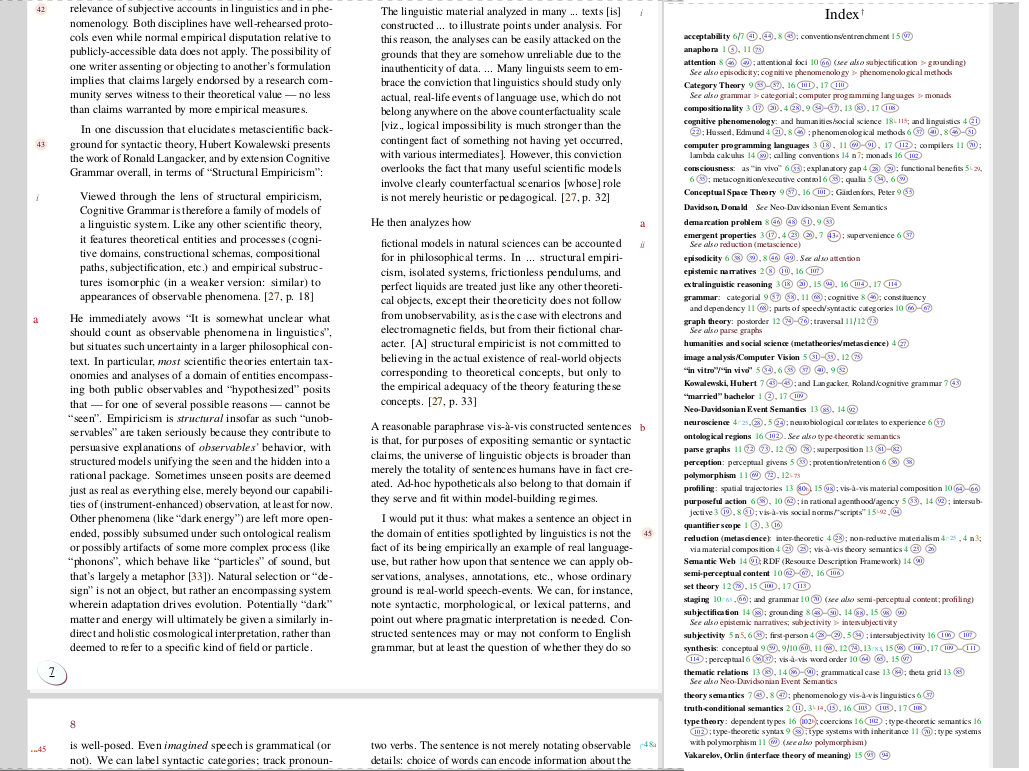
\includegraphics[scale=0.71, trim=0 0 0 0, clip]{x/xNC.png}
\caption{Subdivision formats for Paragraph IDs}
\label{fig:xNC}
\end{figure}

\clearpage{}

\item[Indexing Digital/Multimedia Repositories]  For 
some initiatives, authors deposit content in a 
variety of media, including but not limited to 
text documents.  For example, the 
Cancer Biomedical Informatics Grid (\CaBIG{}) 
project is an oncology research network 
across multiple continents; institutions can join 
the network if they adhere to \q{Vocabularies and Common Data Elements} 
(\VCDE{}) standards applying to \API{}s, metadata, provenance 
declarations, execution models, and so on, to 
support cross-network interoperability 
(for example, data from one institution could be 
plugged in to simulations from another).  Preparing 
indexes for publications deposited to 
a structured research network such as \CaBIG{} 
(now succeeded by \NCIP{}, the National Cancer Informatics 
Project) optimally includes aligning each 
index with semantic protocols.  For example, index 
entries can be linked to \VCDE{} terms wherever 
possible.  Likewise, text- and index-search \API{}s 
can be subsumed under the research grid \API{} 
policies; the shared versioning system can be 
applied to iterations of a manuscript; and 
and metadata can cross-reference text publications 
with other submissions by the same (or affiliated) authors.  

\pseudoIndent{}  Similarly, according to standards such as 
\FAIR{}data, publishing findable, accessible, 
interoperable, and reusable data sets goes beyond 
just making raw data available on an open-access platform.  
In addition, \FAIR{}data defines documentation and metadata 
protocols, so that each statistical parameter (for example) 
is described with range, measurement, distribution, and 
similar analytic information. 

\pseudoIndent{}  On a scientific grid such as 
\CaBIG{}, many assets are executable code 
for \q{\textit{in silico}} simulations.  
From a user's perspective, however, such 
executables often function as multimedia 
resources, producing two- or three-dimensional 
graphics that are pedagogically analogous 
to image series or videos.  Such computer code 
thereby connects to publications with a 
similar rationale as videos, digital maps, and 
other highly-visual content types.  For instance, 
analysis of habitat regrowth after a forest 
fire can be based on footage of actual locations 
or of agent-oriented simulations that provide 
mathematical models for stages of regeneration 
(which plant and animal species become reestablished 
at which point in time).  Indexing and cross-referencing 
policies that are adapted for image and video material 
can thereby be extended to code libraries as 
well.  Controlled vocabularies and other semantic 
standards apply to the familiar elements 
of computer code --- procedures, classes, data types, 
inheritance/containment hierarchies, pre- and post-conditions, 
etc.\@ --- but in a \q{research grid} context graphical displays 
often function as assets in their own right and can 
be annotated and indexed as such.  A \ThreeD{} simulation, 
for instance, functions essentially as a video whose 
specific frames evolve algorithmically as a product 
of parameters and initial conditions that may 
be modified for each run (indeed, videos could be 
taken directly from dynamically evolving \GUI{} windows; 
see Figure~\ref{fig:pcbi}).
  
\pseudoIndent{}  Disciplines such as systems biology, 
environmental science, quantum cosmology, and neurophysics 
are characterized by research networks that explore complex 
systems from multiple angles, and leverage resources 
combining data, code, graphics, simulations, and natural-language 
text.  \lPacTk{} can help authors expand indexing protocols 
to encompass this wider range of scientific content.  

\pseudoIndent{}  In particular, we propose a \q{\FAIR{}data 
Systems Biology Dialect} (\FSBD{}) to standardize \Cpp{} 
code annotations according to \FAIR{}data principles.  
While not restricted to systems biology, this protocol 
would reflect coding requirements for architectures such 
as \CaBIG{}, with the goal of a unified meta-index 
paradigm encompassing data, code, and 
visual assets on decentralized scientific research grids.
In addition to metadata, \FSBD{} would address 
concerns specific to modular software engineering, 
such as merging component-local changes to a 
common database; discovery, validation, and integration of new modules; 
and reading intracomponent 
annotations to create shared, searchable 
documentation (form fields, user-initiated 
operations, authentication, component capabilities, etc.). 
\enlargethispage{25pt}

%\vspace{15pt}
     
%\setlength{\abovecaptionskip}{-5pt}

\begin{figure}[h!]
\hspace{-25pt}
\includegraphics[scale=.95, trim=0 4cm 0 0, clip]{x/m2m.png}
\caption{Index Search in a PDF Front-End Context}
\label{fig:m2m}
\end{figure}


\clearpage{}


\end{description}
}

\vspace*{-43pt}


\sstitle{PacTk's Proposed \q{FAIRdata Microcomponent Protocol} (FMCP)}

\vspace*{7pt}

\p{In component-oriented programming, the term \q{microcomponent} is 
sometimes used for a visually and functionally isolated part 
of a larger application, such as a single web page within a web site, 
or (in the desktop context) a single application window.  
Modular software can be designed as an aggregate of 
many microcomponents.  When reading publications, for 
example, microcomponents could provide functionality to 
view specific kinds of dynamic graphics connected with 
a manuscript, or review raw data files in an associated data set.}

\p{To illustrate how microcomponent programming affects 
indexing and document-preparation, consider the screenshot 
reproduced in Figure~\ref{fig:oh}, left (taken from the OpenHospital 
user manual).  Although this is part of a \Java{} application, 
a \Qt{} developer could readily implement a \Cpp{} version 
of the same component; assume, then, that in so doing 
we intend to annotate the relevant classes with \FMCP{} metadata.}

\p{In particular, there are numerous areas within the \GUI{} 
window with selections/options that may be connected 
to controlled vocabularies, including the list of 
checkbox labels for test results, and the drop-down 
(combobox) values for \q{material} (note that, in the 
existing code, there is no way to find a list of 
possible entries for this field without running 
the software or examining the \Java{} code directly).  
There are also multiple actions users can perform 
through this component, including finding a patient 
id via their personal info; selecting a from a 
calendar display; and recording exam results 
to a hospital database.  Although these logistic and semantic details may 
be implicit in code documentation or user instructions, 
\FMCP{} employs code annotations to specify this metadata 
in a machine-readable fashion;  
the entire software base can then have a single indexing 
and search entry-point (e.g., a query for the 
term \q{urinanalysis,} should match this microcomponent 
as one option for the exam-type field).  In addition, 
new microcomponents could be added to the hospital software 
systematically.  Consider, for instance, that a more 
specialized exam report is needed for a particular clinical 
trial.  Via microcomponent programming, that special-purpose 
page/dialog box could be integrated, and accessed 
by users, similarly to this generic exam window.}

\p{In the context of a research grid such as \CaBIG{}, 
content from disparate institutions are designed 
to interoperate.  For example, one resource might be a 
Geographic Information Systems (\GIS{}) data set 
tracking carcinogens in air or ground pollution plus 
incidents of different types of cancer; another 
resource might be software specifically designed 
to analyze and display this data (on a digital map).  
Such \GIS{} attribute layers have a domain-specific 
nature that is difficult to accommodate with 
generic software such as \textbf{ArcGIS}.  In particular, 
the \GIS{} data points will represent either incidents 
(or measurements) of carcinogenic contamination or 
cancer diagnoses (organized by tumor classification).  
Apart from being governed by controlled vocabularies, 
such data points would have distinct \GUI{} 
requirements (Figure~\ref{fig:car}).  For instance, 
cancer varieties 
can be a terminological bridge for multiple 
data sets and leveraged via search \API{}s. 
Lists of known carcinogens can likewise 
be incorporated into software that works 
with repositories curated 
by the \EPA{} and other organizations.
In general, context/menubar options, 
check/radio buttons, comboboxes, and  
clickable elements may all be 
indexed according to grid schemas.}

\p{For publishing and indexing, apart from semantic 
metadata such as standard nomenclature and 
\q{Common Data Elements} (defined by \NCIP{}, for 
example), some \GUI{} components (as discussed above) 
may function as graphics displays properly indexed 
as multimedia content.  On the right in Figure~\ref{fig:oh} 
is a screenshot from the Cancer Imaging Phenomics 
Toolkit which has multiple data fields suitable 
for \FMCP{} indexing, including textural segmentation 
and feature-extraction algorithms.  In addition, 
the bioimage displays together with region-of-interest 
markings may function as \q{nanopublication} resources 
on a research grid, particularly with case-study 
examples used to demonstrate analytic methods (as with this 
picture).  Illustrations appearing in publications may 
thereby be linked to microcomponents from which the 
graphics were obtained.}
\enlargethispage{2em}
\vspace{-17pt}

\setlength{\abovecaptionskip}{2pt}

\begin{figure}[h!]
\hspace{-45pt}\raisebox{-6pt}{\includegraphics[page=53, scale=.56, trim=0 11cm 0 0, clip]{UserManual.pdf}}%
\hspace{-18pt}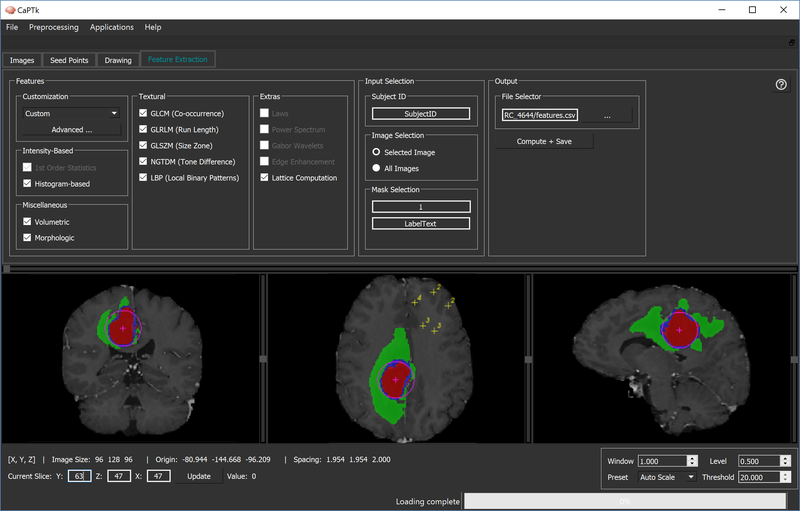
\includegraphics[scale=1.1, trim=0 3cm 0 1cm, clip]{baseScreenshot.png}
\caption{OpenHospital form (left) and cancer imaging window (right) 
as microcomponent examples}
\label{fig:oh}
\end{figure}


\clearpage{}

\setlength{\abovecaptionskip}{9pt}

\vspace*{-6em}
\sstitle{Grid Architecture According to FAIR Principles}

\vspace*{15pt}

\p{Grid Computing is an important part of contemporary scientific 
research.  In general, a \q{grid} --- in contrast to a 
just data-sharing network --- combines data, code, and multimedia 
content.  More specifically, a grid is designed with the assumption 
that users will execute software packages which are accessible 
via the grid, and that their primary reason for doing so is 
because the software encapsulates novel research: 
quantitative or qualitative (e.g., agent-based) simulations, 
\q{in silico} experiments, analysis of newly-available empirical data, 
algorithmically generated graphics, and so forth.}

\p{In some instances, code packages may be downloaded and run privately, 
e.g., on a scientist's own computer.  In other cases, the code 
specifically requires special hardware (e.g., supercomputing/massive 
parallelization) and a grid enables researchers to execute remotely, 
on computing nodes that have the requisite capabilities.}  

\p{It would be a mistake, however, to assume that grid computing 
necessarily involves technologies that require atypical 
execution environments.  Instead, grid principles can 
overlap with \FAIR{} priorities, because openly sharing 
simulations and analyses is one dimension of research 
transparency.  Given a simulation with specific 
initial parameters, for example, any interested 
scientist should be able to execute the code 
themselves and achieve the same results (or, 
if probabilistic/stochastic methods are involved, at least 
\textit{similar} results).  Moreover, variations 
in initial conditions should affect simulation 
output in predictable (or at least explainable) ways.}

\p{There is also a pedagogical value in running and examining 
simulation and/or analytic code.  Academic papers often 
present research methods in abstract, mathematical terms; 
observing visuals and experimenting with code 
parameters can help make the underlying research 
more understandable.  This inures to the benefit 
of scientists who wish to assess (and perhaps 
replicate) published research, as well as students 
who might use specific experiments or investigations 
as tools to learn about their ambient disciplines.} 

\p{With this in mind, we can formulate several 
core principles of \q{\FAIR{}} grid computing, 
including: \textbullet{} code packages hosted 
on a grid should be designed with as few 
mandatory external dependencies as possible; 
\textbullet{} where a given package has software 
or hardware requirements that are difficult to 
satisfy, a simplified version should be made 
available that would at least allow some 
provisional learning and evaluation of published 
results; \textbullet{} every effort should be 
made to ensure that the software executes in a 
usable fashion even in the absense of dependencies 
or preconditions that held true for those developing 
the code; and \textbullet{} there should be a 
clear set of actions, with as few steps as 
possible, allowing someone newly acquainted 
with a grid-hosted package --- in particular, someone 
who learns about the code from a technical publication 
--- to obtain and execute the relevant code.  
In particular, they should be able to build and 
use the software in parallel with figures and 
text discussions featured in document manuscripts.}

\p{The following are several examples of how a properly 
\FAIR{} grid might work, which are paired 
with \q{counter-examples} that discuss lacunae 
in \textit{existing} implementations of research networks.}

\begin{description}

\item[Computer Simulations and Videos]  A publication presents a 
new \q{in silico} investigation, such as the simulation of 
interrelated biological processes on a cellular or tissue scale.  
The paper includes frames from a simulation video and 
supplemental materials link to the video in its entirety.  
The video itself records the output of a particular run of 
the simulation, with a given set of initial conditions.

\pseudoIndent{} 
  

\item[GIS Attribute Layers Reflecting Multiple Scientific Disciplines]

\item[Curating Corpora of Linguistics Examples]

\item[A Modular EMR System]




\end{description}

\clearpage{}


\vspace*{-43pt}

{\semihr{0.647\textwidth}}
\vspace*{5pt}
\hspace{2pt}\secttitle{{Extending Beyond Single 
Documents: Data Transparency and Translational 
Science}}\sstitletri{7}\sstitletri{2}\sstitletri{2}
\vspace*{5pt}
{\semihr{0.647\textwidth}}

\vspace*{9pt}

%\setlength{\footskip}{2pt}
%\p{}

\p{Rethinking the relationship between pure and applied 
research, between universities and communities, 
means a changing landscape for publishers as well.
Although all biomedical research (and scientific work in general) 
is motivated in principle by practical benefits, translational 
emphases promote the institutional and informatics foundations 
for \q{bench to bedside} translation to happen   
as quickly and comprehensively as possible.  
Scholars in the field of \q{translational science,} for 
example, have developed a five-part model of the 
evolution of practical interventions %,\footnote{\hspace*{4pt}
(also 
called the \q{translational continuum}; see 
for instance \href{https://www.iths.org/investigators/definitions/translational-research}
{https://www.iths.org/investigators/definitions/translational-research}) %}
of which the 
fourth involves commonplace adoption of (once-)novel 
practices in clinical settings and the fifth 
marks concerted efforts to adopt useful 
interventions in a wide variety of settings 
(e.g., not restricted to protocols 
available only in a few hospitals).  
Such models suggest roadmaps to help 
guide deployment once research progresses through  
multiple stages of concrete imple- mentation.  Published materials 
(not necessarily restricted to journal articles) 
may reflect data and observations at each of these stages.}

\p{Apart from theoretical models along these lines, the 
key details of translational deployment are often 
institutional and socioeconomic in nature.  
Sustaining research projects enough to 
rigorously assess empirical outcomes is a different 
process than procuring funding, labs, and teams 
to work through initial objectives on 
purely scientific grounds.  Some innovative 
software initiatives (e.g., the \CaBIG{} \DMR{} 
mentioned above) were discontinued; other 
frameworks, such as 
the University of Pennsylvania's Cancer Phenomics 
Toolkit, evince novel biocomputational ideas but have not been 
scaled up or replicated beyond their academic point of origin.  
These suggest fortuitous connections between 
technical and translational priorities.  Further development 
and adoption of promising 
software, interventions, or clinical protocols can 
be spurred by goals 
to make effective health care options 
(for example) available to a broad spectrum of 
the community.  Research initially supported on purely 
technical grounds might 
then further expand 
by emphasizing social/translational benefits.} 

\p{From a publishing standpoint, translational science 
implies that a research infrastructure should sustain and 
evolve over multiple phases of a scientific project, 
which extends beyond the time-frame of individual 
books or articles.  This is reflected in part by 
protocols such as \q{Research Objects} where supplemental 
materials (graphics, data sets, utility computer code, and so on) are presented 
in standardized ways.  It is also manifest 
in notions of replication and data transparency: 
models such as Minimum Information Standards 
that illustrate experimental/data-acquisition modalities to facilitate 
subsequent investigations confirming or extending the 
scope of published work.}

\p{More broadly, translational priorities imply that 
variegated stakeholders --- not only scientists 
but also practitioners, funders, government representatives, 
etc. --- are best served by integrated packages describing 
the scope, goals, and (possibly intermediate) results of research 
projects.  In current practice, multiple files and resources 
associated with academic publications are often scattered 
in different places, without clear provenance or interoperation.  
Specifications such as the Research Object protocol only 
partially alleviate this problem.}  

\p{Against this background, \PacTk{} proposes a \q{Translational Research Object 
Protocol} that honors the goals of both Research Objects 
(as a paradigm for dissemination of scientific works) 
and Translational Science (as a collation of best 
practices for emphasizing social benefits of research innovations).
According to this protocol, individual publications 
exist in the context of \q{Project Archives} that have 
singular entry points both online (potentially 
integrated with publishers' search portals) and 
through downloadable resources/data sets.  
Materials associated with a publication, aggregated through this entry 
point, would summarize translational 
possibilities for the documented research 
and provide a foundation for institutional 
deployment(s).  Individual scientists or students 
could also utilize Project Archives as encapsulations 
introducing their interests, background, and expertise 
to fellow researchers as well as those 
whose responsibilities include assessing the 
merits and adaptation potential of projects 
originating in academic (as well as private/independent) 
environments.}

%\vspace{11pt}
 

%\clearpage{}

%\begin{figure}[h!]
%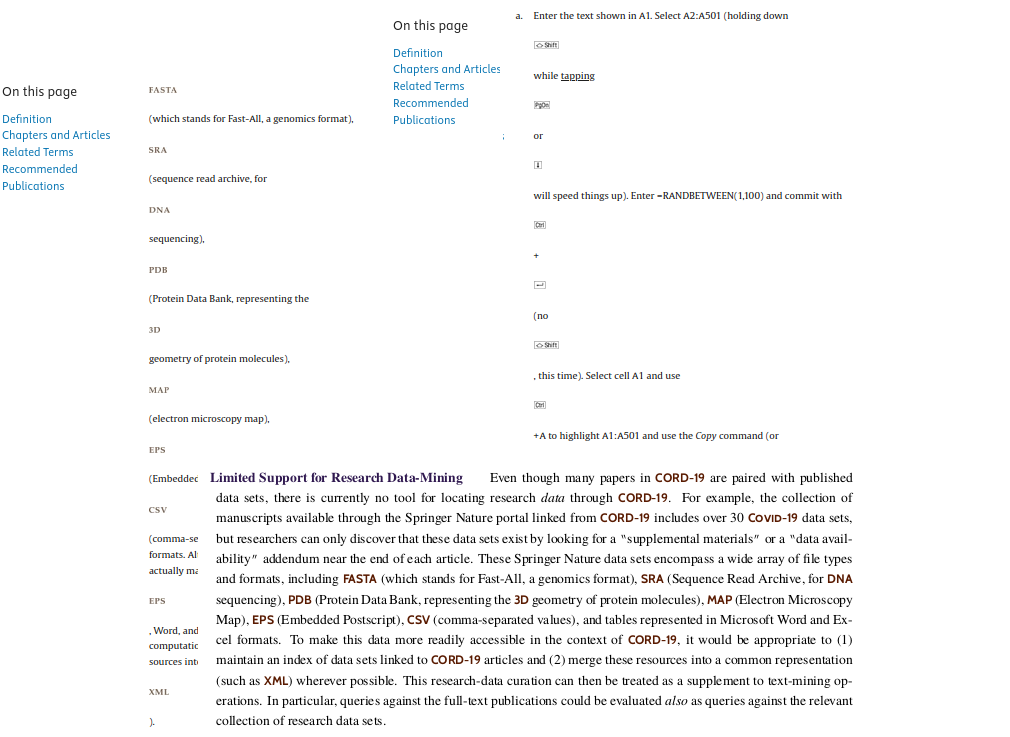
\includegraphics[scale=0.71, trim=0 0 0 0, clip]{x/x2.png}
%\caption{HTML Transcription Errors}
%\label{fig:ss6a}
%\end{figure}

%\sstitle{Constraint Declarations and Other VM Use-Cases}

%\pagebreak{}\newpage{}\clearpage{}

\vspace*{-4pt}

\sstitle{Data Publishing and Multimedia}


\vspace*{8pt}

\p{Contemporary data transparency and \FAIRsharing{} 
(Findable, Accessible, Interoperable, Reusable) standards 
introduce new challenges for publishers.  In this environment, 
published documents such as \PDF{}s serve as only 
one part of a package of files, alongside research data 
sets and, often, numerous forms of multimedia content 
(potentially including audio, video, image series, \ThreeD{} graphics, 
and statistical/data-visualization tools and diagrams, plus domain-specific 
interactive formats).  If desired, 
\PDF{} viewers could themselves be implemented as one 
portion of a multimedia suite, with functional motifs 
duplicated across the various components (Figures~\ref{fig:ss8}~and~\ref{fig:ss9}).}

\setlength{\belowcaptionskip}{5pt}

\begin{figure}[t!]

\includegraphics[scale=0.5]{fin/stark-mi.png}
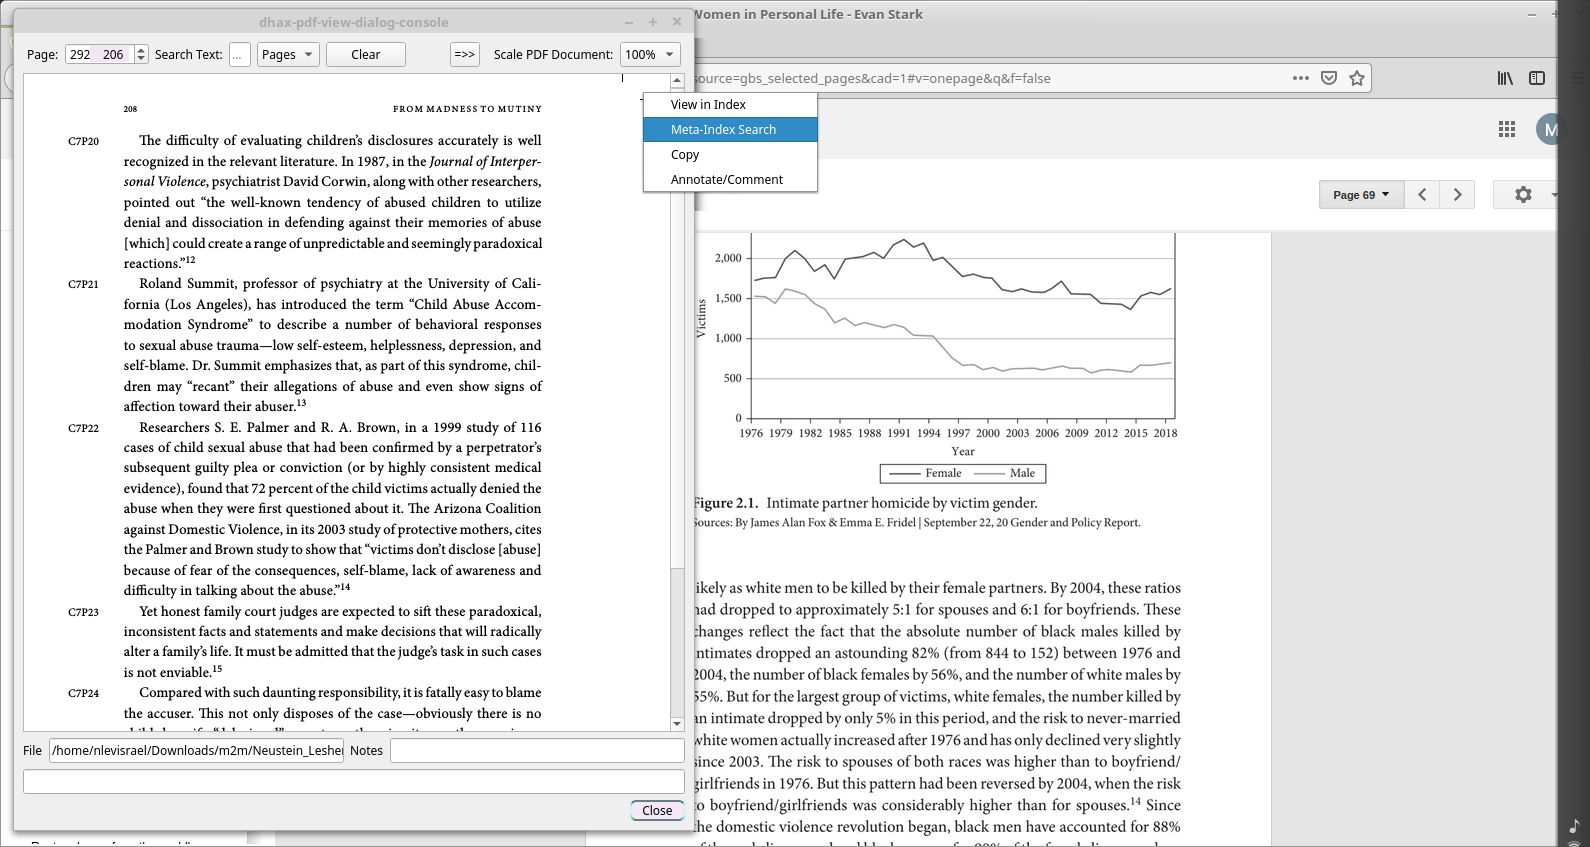
\includegraphics[scale=0.5]{fin/stark.png}
\caption{Meta-index search through a web portal}
\label{fig:ss7}
\end{figure}


\setlength{\belowcaptionskip}{0pt}

\p{As a \q{publishing accelerator} toolkit, \PacTk{} has 
several components to help publishers construct these 
supplemental materials, including cross-referencing 
text documents with associated data/media assets, and 
ensuring \FAIR{} usability.  Here are several 
examples:%\enlargethispage{1em}

\begin{description}

\item[Deserialization and Dataset Tools]  Individual scientific disciplines are often 
associated with domain-specific data publishing formats that are paired with 
dedicated deserialization tools (i.e., computer code that 
reads raw data files into live memory, without relying on special-purpose 
software).  Such code libraries are often maintained by individual 
institutions or organizations --- which might be academic departments, research 
labs, or independent groups --- on behalf of a 
broader research community.  Examples include (among many) \FASTQ{} and \VCF{} for genomics; \HDFfive{} and \ROOT{} for physics; 
\FITS{} and \netCDF{} (astronomy and earth sciences); \PDB{}, \MOL{}, 
\SBML{}, and \CELLML{} (biochemistry); 
\IFC{} and \BIM{} (architecture/engineering); \SEGY{} and \BAG{} 
(geophysics and oceanography); \CoNLLU{} (computational linguistics); 
\DICOM{} and \OMETIFF{} (bioimaging); and \GIS{}-indexed attribute layers 
and shapefiles for geospatial data sets.

\pseudoIndent{} Some domain-specific file formats are derived from general-purpose 
specifications such as \XML{}, \CSV{}, and \JSON{}.  Others 
employ idiosyncratic text and/or binary 
serialization protocols, so that custom parsers are necessary so as to consume byte or character 
streams from relevant raw data files.  Even when the actual encoding is performed via a 
generic standard like \XML{}, dedicated deserialization code will still be needed --- 
ordinary parsers may convert a given \XML{} document to a %Document Object Model 
\DOM{} infoset, but extraction algorithms 
still must navigate the document hierarchy and obtain 
text strings from element nodes, which become the input for initializing 
object data fields.

%\newpage{}\clearpage{}
\pseudoIndent{} \lPacTk{} seeks to address these issues by offering a 
platform-independent Virtual Machine that is easy to host within 
scientific applications or build as a plugin or standalone program.  
Scripting 
or query languages can then emit code for this \VM{} to 
take responsibility for deserializing encoded data sets 
(while, as another use-case, the \VM{} could be embedded in 
\Cpp{} classes/microcomponents   
as a runtime contract-verification tool).  Depending 
on format, \VM{} instructions might navigate through 
graph-like structures in a standardized profile (like \XML{}) 
or implement and/or integrate with parsers for custom input file types, 
through postprocessors or rule-match callbacks.  

\pseudoIndent{} Via these technologies, publishers may ensure that 
data sets are accessible so long as there are deserialization 
libraries targeting a \PacTk{} \VM{}, rather than duplicating 
effort (requiring multiple libraries for different operating 
systems and programming environments).\vspace{6pt}  
 
\begin{figure}[ht]
\hspace*{1em}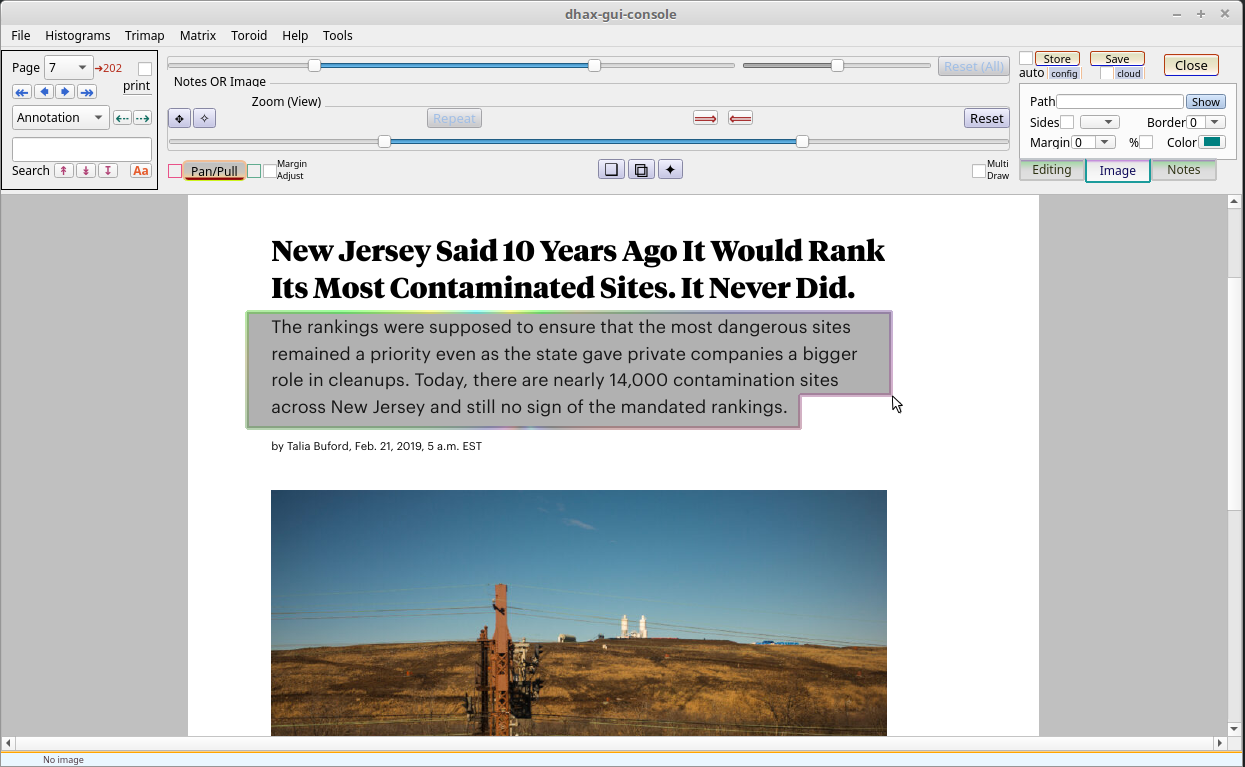
\includegraphics[scale=0.47, 
trim=0 12pt 0 22pt, clip]{fin/oct.png}
\caption{Flexible range-select features}
\label{fig:ss8}
\end{figure}

\vspace{1pt}

\item[Analytic and Demonstrative Code]  Many data sets are published 
alongside copies or samples of code used to analyze the raw data.  
Code sharing is important for transparency (allowing outsiders 
to double-check the accuracy of calculations and conclusions 
drawn therefrom) and reuse (replication of experiments/research projects).  
Data publications (bundled as Research Objects or similar scientific 
packages) may also include implementations for plugins targeted at 
applications charged with loading the raw data files.  
\lPacTk{}'s object system includes several classes encapsulating 
plugin functionality (such as dynamic-library symbol resolution) 
and components exposed by host applications to extension 
modules (main-window taskbars, top/context menus, 
filesystem access, etc.).
  
\pseudoIndent{} Although such accompanying code might be implemented 
in many different languages and environments, the \VM{} principles 
identified above for deserialization tasks also apply 
to code specific to research data sets.  Here, too, accessibility 
implies that dataset code should be available in a cross-platform 
manner.  Broadly-usable code libraries for (e.g.) deserialization 
obviate the need to achieve interoperability via reified/canonical  
model-representation standards alone.  For example, 
Semantic Web nodes could be annotated with information about 
libraries that could unpack objects whose data fields 
supply values to nearby sites in the node's shape-constrained 
neighborhood.  Moreover, implementations should proceed via 
conventions suitable for \GUI{} wrappers and interop (in particular, 
microcomponent protocols described earlier) because 
research methods will often rely on domain-specific 
scientific or academic software.  Ideally, users will examine data 
sets with the aid of plugins for applications familiar to 
the relevant research community, or at least custom-built 
software that can interoperate with those domain-specific technologies.  
Unfortunately, many of the most popular scripting formats 
in scientific/research contexts (e.g., \Python{}, \JavaScript{}, and \R{}) 
have noticeable limitations \visavis{} native-\GUI{} integration.  

\pseudoIndent{} \lPacTk{} enables a different approach, wherein 
languages can be customized to individual data sets and target 
pure-\Cpp{} \VM{}s whose entire parsing, \IR{}, and runtime stack 
is embeddable (as source files) in \Cpp{} \GUI{} applications with no outside 
dependencies.  Compilers and runtime engines for dataset code may 
thereby be released as part of the publication package itself.  
The \VM{} and peer components could also be built directly 
into \PDF{} viewers, multimedia applications (for videos, digital 
maps, etc.), and scientific computing platforms.

\pseudoIndent{} Another \PacTk{} benefit for dataset code involves 
documentation and pedagogical features.  In these contexts, code 
serves not merely to derive specific computations but also 
to demonstrate the acquisition methods and analytic protocols relevant 
for a research project.  Such details as units of measurement, 
expected ranges, typed coordinate systems (e.g., ensuring that 
procedures expecting horizontal-then-vertical coordinate 
pairs are never called with the converse), 
compile-time/statically-analyzable pre- and post-conditions, and so forth, 
help dataset code to serve as a resource clarifying scientific 
principles and theoretical models that drive published findings.  
The \PacTk{} Virtual Machine includes overload-by-contract, 
dependent typing 
(a version thereof compatible with template metaprogramming, as such 
with some technical differences from, say, \Idris{}), native 
interop (with statically compiled as well as dynamically loaded libraries) 
and \q{user-defined} calling-convention features that differ 
in some technical details from typical language interpreters, 
resulting in a scripting environment specifically built for 
open-access data sharing and the deployment of data packages 
as pedagogical tools.    


%\begin{figure}[ht]
%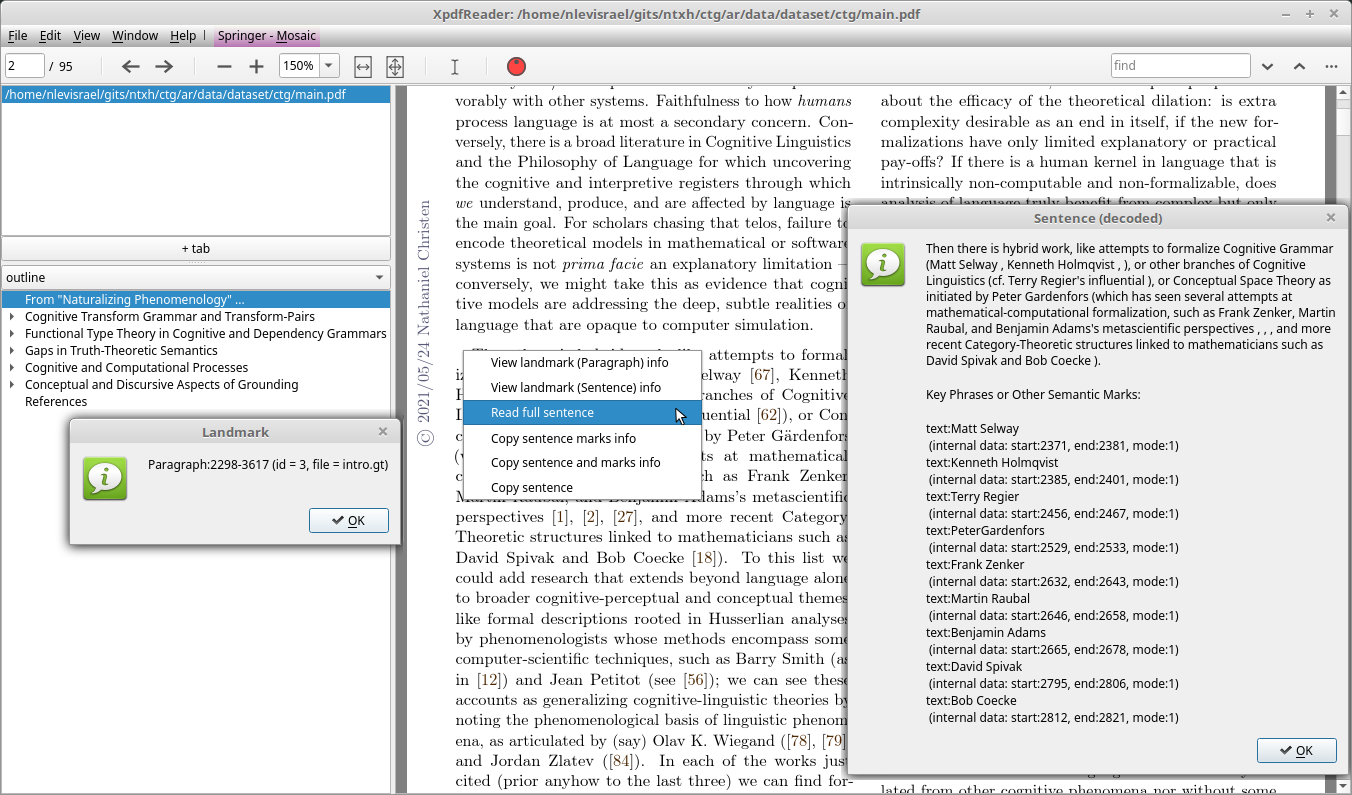
\includegraphics[scale=0.45]{fin/ling.png}
%\caption{Enhanced GUI capabilities enabled by machine-readable text encoding}
%\label{fig:ss8}
%\end{figure}

\vspace*{8pt}

\begin{figure}[h!]
\hspace{18pt}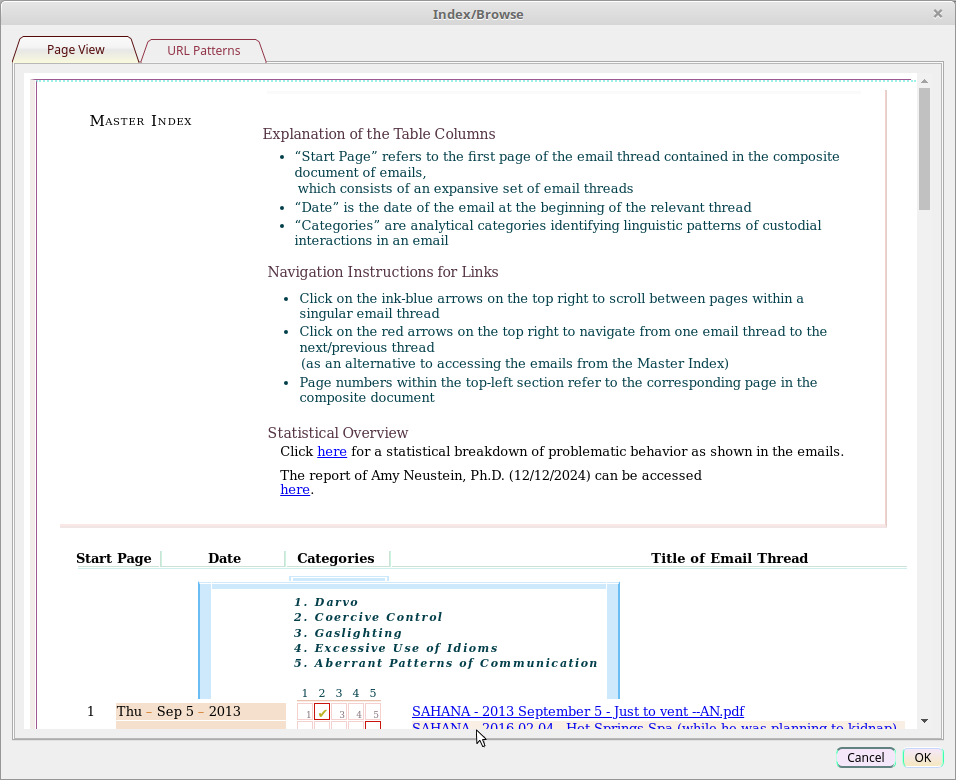
\includegraphics[scale=0.5, trim=0 2mm 0 6mm, clip]{fin/sah.png}
\caption{A category-based web-accessible index table for SVG pages}
\label{fig:ss9}
\end{figure}

\vspace*{-4pt}

\item[Full-Text Query Languages]  As discussed earlier in this 
document, \PacTk{} can be utilized as a code library by 
calling methods on \Cpp{} (specifically, \TSOM{}) objects.  
At the same time, a \PacTk{} Virtual Machine supplies an  
environment for compiling scripting or query languages.  
These functionalities could be merged, such that the process 
of extracting information from a \PDF{} manuscript, 
meta-indexed repository, or bibliographic database might be 
achieved by formulating and evaluating part of the code in a 
specialized query language.  The techniques involved 
would be similar to employing \XQuery{} or \XQSE{} 
expressions to work with \JATS{} or \BITS{} files.

\pseudoIndent{} \lPacTk{} features its own flexible front-end parsing 
framework (mentioned above relative to \GTagML{}) that 
could be used to program query grammars in an extensible, 
adaptable manner.  By leveraging full regular expression 
capabilities, callbacks to arbitrary code (instead of 
generative production rules), and directly-executable 
grammar files (with no separate compilation steps), 
the \PacTk{} parsers are more flexible than conventional 
\LEX{}/\YACC{}-style compilers.  Meanwhile, the \VM{} 
runtimes allows query evaluators to recognize basic 
scripting constructions such as locally-scoped variables 
and calls to arbitrary boolean-valued procedures as 
filter parameters.

\pseudoIndent{} In totality, such features allow 
text/bibliographic query systems to be implemented 
in a self-contained and cross-platform manner, 
with customizations specific to individual publishers 
and even to each particular journal or book series.  

\vspace*{-4pt}


\item[Multimedia Cross-Referencing]  When a document (book or article) is explicitly paired with a 
published data set, information about the supplemental package should be 
included in index/search metadata.  This would allow 
keyword searches to be extended to raw data fields, as well 
as data-structure parameters (column labels, source-code 
annotations, procedure names, etc.).  Moreover, sections of text 
may be isolated as cross-reference targets for data-structure parameters 
as well as individual objects/records.  For example, a specific 
column or field in tabular data structures can be cross-referenced 
with the paragraph in article text where that field is 
discussed (its observation/acquisition methodology, units of measurement, 
valid range delineation, statistical distribution, and so forth).

\pseudoIndent{} Cross-referencing between research papers and data sets 
is a special case of multimedia cross-referencing, where annotations defined 
in the context of a specific media type assert semantic or thematic 
relations to contents of a different modality.  Concrete examples 
of multimedia cross-referencing include geotagging video frames; linking 
\CAD{} digital twins with product specs; annotating Regions of Interest 
within image series with coded labels associated with published raw data; 
information within natural/social science cross-disciplinary areas such as medical 
humanities, translational sciences, socio-agronomics, and civil engineering;
embedding tags in 360\textdegree{} displays whose content includes 
\URL{} strings that encode identifiers for dataset objects; developing 
color- and/or shape-coded attribute layers for \GIS{} overlays (so users 
can browse between digital maps and structured object 
displays); and constructing numeric tuples from \ThreeD{} graphics scenes 
such that particular camera orientation/location and zoom levels 
could be recorded as a unit, allowing relevant \ThreeD{} content to be 
repeatedly visualized from an identical perspective (in other words, 
links are embedded in \PDF{} files, web pages, software, or any 
other context so that users can reconstruct a specific \ThreeD{} state, 
as constituted by camera angle/position and zoom settings).

\pseudoIndent{}  The challenge when implementing multimedia cross-references is to 
ensure that viewers for two or more divergent media types may properly 
interoperate.  With correctly interpreted cross-references, application users should be able 
to navigate from a window dedicated to one media/file to a 
window rendering a different format, and correctly isolate the 
portion of a file (not just the overall file) implicated in a cross-reference.  
For example, geotagging video frames should enable users to pause a video 
at a particular location and then, via the geotag, switch to a map 
display centered on the geospatial coordinates visible in the video 
(consider videos documenting progress in an environmental 
remediation site; or infrastructural and socioeconomic implications of 
Zoning and Land Use ordinances).  Conversely, a \GIS{} attribute layer could represent 
locations for which video content is available, allowing users 
to watch the relevant videos starting from the appropriate time-point.  
Such interoperability is only possible if the components and/or applications 
responsible for rendering the two content-types share a common 
annotation and message-passing protocol.  In the context of \PacTk{}, 
this may be achieved via \TSOM{} \q{message} objects that encapsulate 
remote-method requests and parameter serialization via 
\TagML{}-like structures.
 

\item[Science and Humanities GUIs]   Data publishing 
according to \FAIRsharing{} standards often requires 
numerous project-specific resources in addition 
to raw data files.  Fellow researchers typically 
need visualization and computational tools to 
fully leverage published data sets for 
evaluation and re-use.  Unfortunately, relying on generic 
software to access published information packages is often 
suboptimal.  For example, \CSV{} files might be 
loaded into spreadsheets and/or statistical applications, 
but simply viewing data files in tabular fashion 
(even if the information is conducive to such structures) 
provides only limited value.  The same is true for 
statistical plots and diagrams.  Effective evaluation 
and re-use involves front-end programs that could provide 
both visual overviews (e.g., via charts, graphs, or histograms) 
and functionality for examining individual data objects 
in detail (e.g., via custom-designed \GUI{} windows).

\pseudoIndent{}  Furthermore, many data sets span multiple 
structural profiles.  For example, consider information 
tracking environmental pollutants, such as published 
by the Environmental Protection Agency's 
Toxic Release Inventory (\TRI{}) project.
Software tools for rigorously studying and analyzing such data could 
furnish both \GIS{} maps (for understanding 
geospatial details and patterns about where environmental 
hazards are present) and (bio)chemical software 
for molecular visualization, or other features to 
help document public-health and eco\-logical 
consequences, plus cleanup/remediation protocols for 
different classes of contaminants.  Such components 
might be further ex- tended by economic data 
profiling social impacts on surrounding communities, 
public health information, video and image series. etc.

\pseudoIndent{}  In general, then, publishers should not 
assume that \FAIR{} transparency is achieved simply by 
sharing raw data files.  Instead, open-access materials should 
in general include plugins or source-code extensions (developed 
individually for one manuscript; or collectively 
for a book series, journal title, or document repository) 
targeting science applications with requisite capabilities 
to view/analyze domain-specific file types.  Similar 
comments apply to humanities environments, such as 
front-ends for studying linguistics corpora and/or 
parse-structures; sociological/economic 
statistics; or graphics tools for digital humanities.
\lPacTk{} can help in this context 
because a single \PacTk{} plugin could serve as middleware 
on top of which extensions could operate that are individualized 
to specific publications/manuscripts.  This may be more 
efficient than building components against applications' 
native plugin mechanisms directly. 

\end{description}

}

%\newgeometry{bottom=.7in}


%\p{}
%\p{}

\vspace*{-21pt}

%{\semihr{0.164\textwidth}}
%\vspace*{4pt}
%\sectnum{1.}
%\hspace*{-28pt}\secttitle{{Video Links}}\sstitletri{7}\sstitletri{2}\sstitletri{2}
%\vspace*{4pt}
%{\semihr{0.164\textwidth}}

\sstitle{Video Links}

\vspace*{3pt}

\p{For more information, please see our software demo videos, which show 
software components that could be integrated into dataset applications 
and \PDF{} viewers:

\vspace*{14pt}

% \href{http://www.lingtechsys.com/videos/qmt-composite.mkv}{\parbox{.3\textwidth}{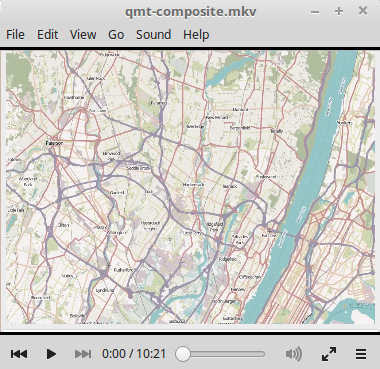
\includegraphics[scale=.3]{pm/qmt-composite.png}\\\GIS{}}}%
% \hspace{10pt}\href{http://www.lingtechsys.com/videos/dhax-composite.mkv}{\parbox{.3\textwidth}{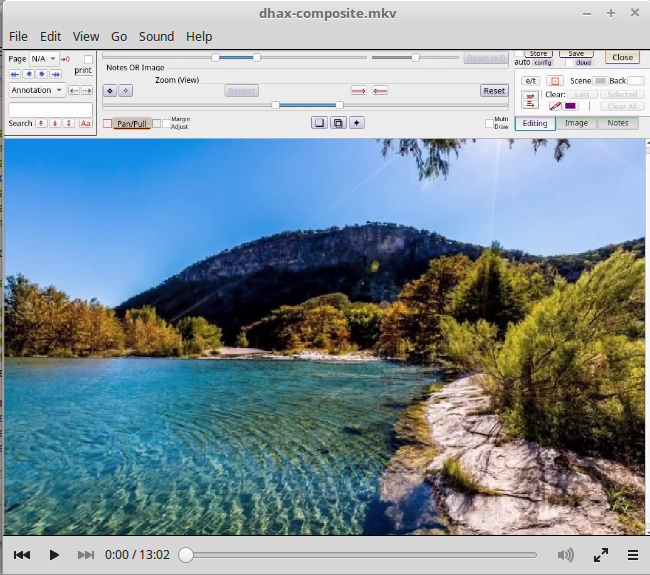
\includegraphics[scale=.255]{pm/dhax-composite.png}\\360\textdegree{} photography}}%
% \hspace{25pt}\href{http://www.lingtechsys.com/videos/xcsd-composite.mkv}{\parbox{.3\textwidth}{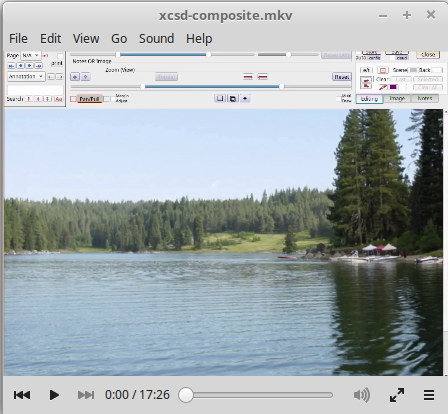
\includegraphics[scale=.35]{pm/xcsd-composite.png}\\Image Processing}}%

}


%\vspace*{3pt}

\pagestyle{lastpage}
%

\clearpage{}

\vspace*{-40pt}

{\semihr{0.2695\textwidth}}
\vspace*{5pt}
\hspace{2pt}\secttitle{{Addendum: Quotations of Interest}}\sstitletri{7}\sstitletri{2}\sstitletri{2}
\vspace*{5pt}
{\semihr{0.2695\textwidth}}

\vspace{9pt}

\begin{displayquote}

Researchers cannot readily search across multiple repositories to find models of interest, and when a researcher does retrieve a relevant model, they must determine whether it (or part of it) can be repurposed for use in their modeling work. Similarity measures and pattern-matching algorithms can help identify relevant modeling components, but existing proposals for cross-repository search and retrieval are mostly theoretical and not yet applicable in practice. Applying semantic annotations in a standardized way across model repositories would provide a common ground for such cross-repository searches, allowing models encoded in diverse formats to be retrieved based on their shared semantic descriptions. 

The amount of time required to select a model for reuse increases when the researcher must choose from a large set of potentially usable models. With only limited means to compare models automatically, researchers must manually assess the content, scope and underlying assumptions of each candidate model as well as the biological questions each was designed to answer. While semantic annotations cannot yet capture the purpose for which a model was built or modified, they can make the biological content of a model explicit and therefore help researchers decide whether or not to repurpose it....

An additional impediment to model reuse is the lack of integration between model repositories and online collections of experimental data. If such integration existed, modelers could readily find data appropriate for validating or constraining the models they repurpose, and experimentalists could find models for use in data analysis pipelines. 

\vspace{-2pt}
\hfill\q{Harmonizing semantic annotations for computational models in biology}

\vspace{-2pt}
\hfill\href{https://pmc.ncbi.nlm.nih.gov/articles/PMC6433895/}{https://pmc.ncbi.nlm.nih.gov/articles/PMC6433895/}

\end{displayquote}

\vspace{1pt}


\begin{displayquote}

\textbf{Call to action}

Though the full text of many scientific papers are
available to researchers through CORD-19, a number of 
challenges prevent easy application of NLP
and text mining techniques to these papers. First,
the primary distribution format of scientific papers
--- PDF --- is not amenable to text processing. The
PDF file format is designed to share electronic documents rendered faithfully for reading and printing, and mixes visual with semantic information.
Significant effort is needed to coerce PDF into a
format more amenable to text mining, such as JATS
XML,26 BioC (Comeau et al., 2019), or S2ORC
JSON ... [W]e can still benefit from better PDF parsing tools
for scientific documents. As a complement, 
scientific papers should also be made available in a
structured format like JSON, XML, or HTML.

\vspace{-2pt}
\hfill\q{CORD-19: The COVID-19 Open Research Dataset}

\vspace{-2pt}
\hfill\href{https://aclanthology.org/2020.nlpcovid19-acl.1.pdf}{https://aclanthology.org/2020.nlpcovid19-acl.1.pdf}

\end{displayquote}

\definecolor{rray}{RGB}{161, 110, 52}
\definecolor{rgray}{RGB}{200, 107, 49}


\textcolor{rgray}{\hrule}
\vspace{1pt}
\textcolor{rray}{\hrule}
\vspace{1pt}
\textcolor{rgray}{\hrule}

\enlargethispage{3em}

\vspace*{-26pt}

\begin{figure}[h!]
\hspace{125pt}\includegraphics[page=5, scale=.85, trim=0 13.4cm 0 0, clip]{x/pcbi_1002970.pdf}%
\vspace{3em}
\caption{Potential locations for code/data/multimedia cross-reference annotations}
\label{fig:pcbi}
\end{figure}


\clearpage{}



\begin{figure}[h!]
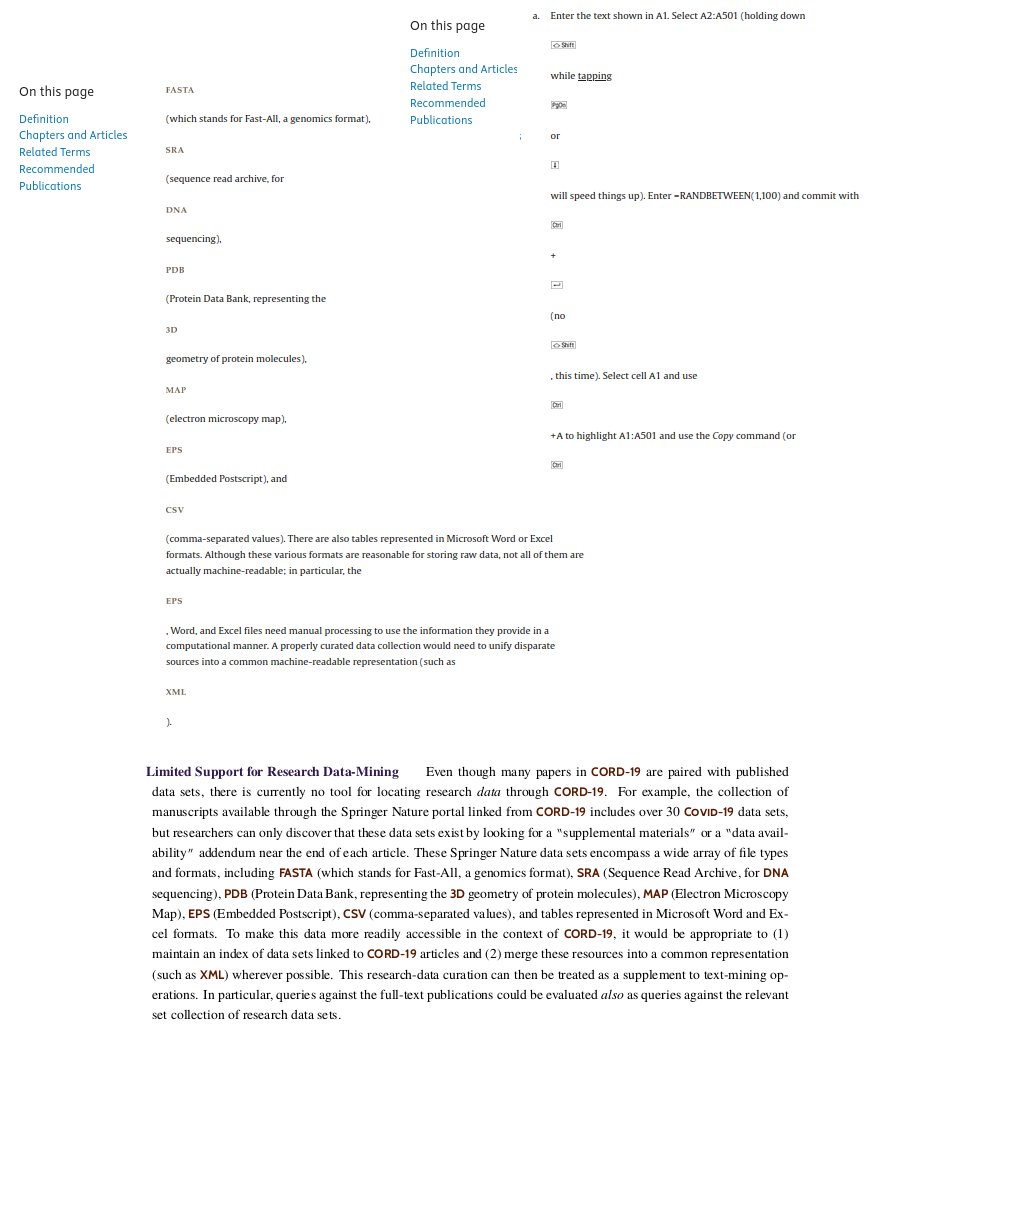
\includegraphics[scale=0.71, trim=0 0 0 0, clip]{x/x3.png}
\caption{HTML Transcription Errors}
\label{fig:ss10}
\end{figure}


\clearpage{}



\begin{figure}[h!]
\hspace{-25pt}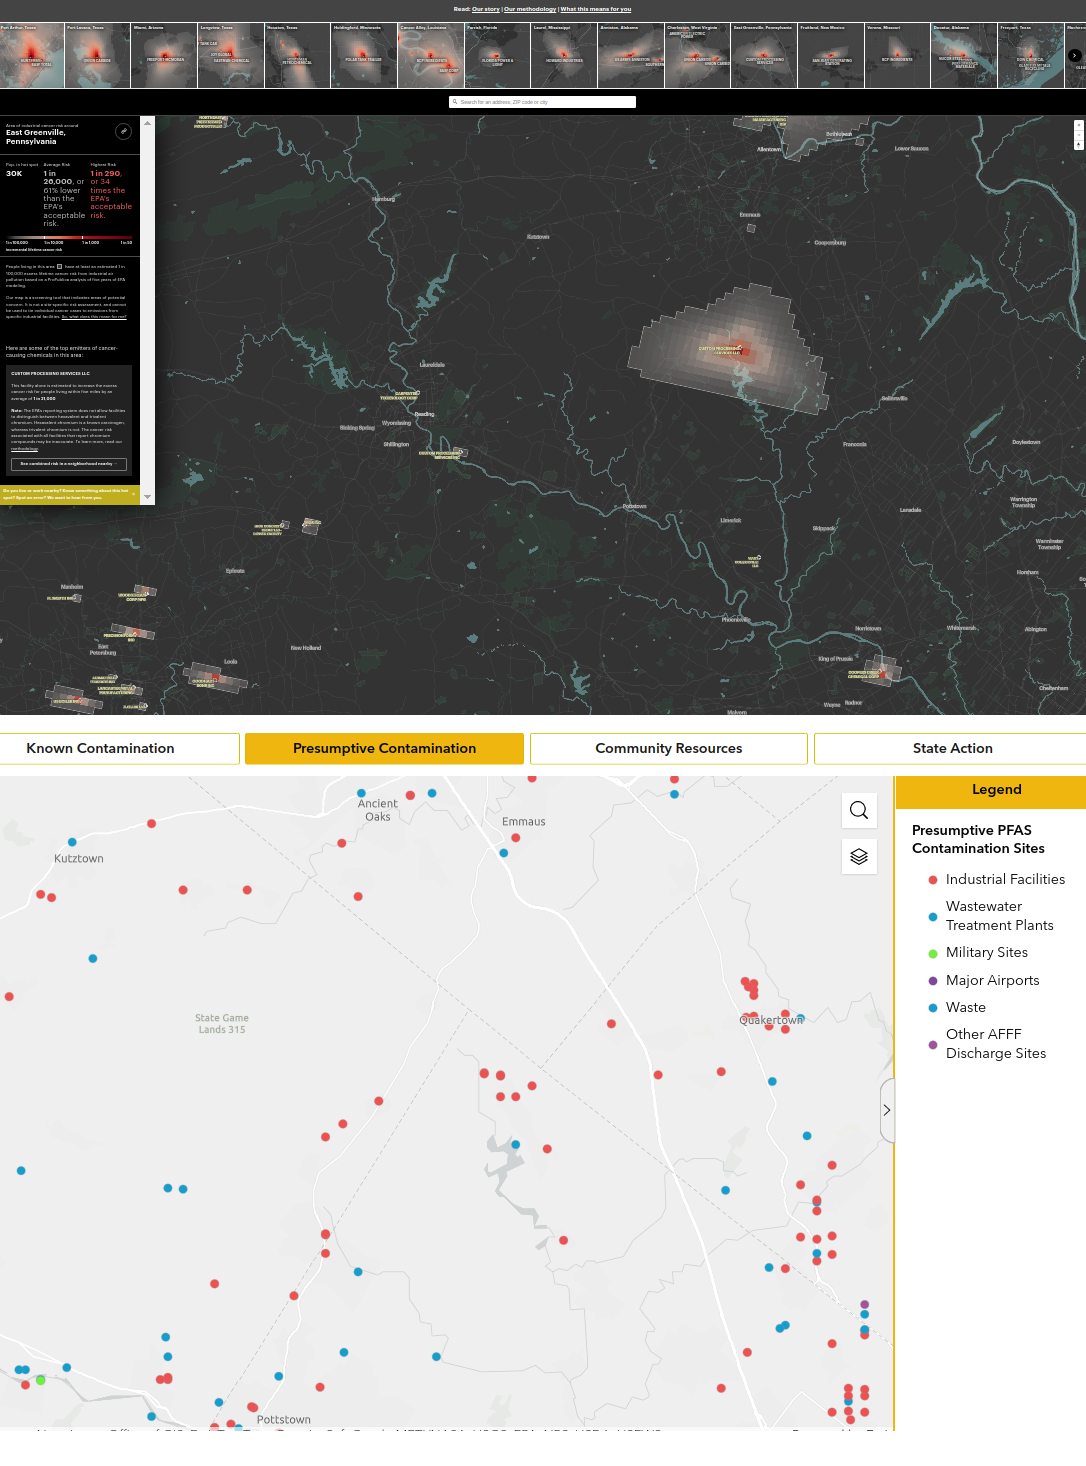
\includegraphics[scale=0.61, trim=0 1.3cm 0 0, clip]{x/car/car.png}
\caption{GIS/Public Health Interoperability}
\label{fig:car}
\end{figure}




%x/

%\p{}


\end{document}

% Figure 1  ZoLa compared with a static \PDF{} map
% Figure 2  Merging NYC environment-related classifications 
 %            with WRI and ISI designations
% Figure 3  Custom query windows for accessing E-Designation data
% Figure 4  Customizable basemaps and data-layer overlays
% Figure 5  Managing communications with NYCPlanning \API{}s as part 
 %            of a metro area-wide \API{} integration 




